%  LaTeX support: latex@mdpi.com 
%  In case you need support, please attach all files that are necessary for compiling as well as the log file, and specify the details of your LaTeX setup (which operating system and LaTeX version / tools you are using).

%=================================================================
\documentclass[sensors,article,submit,moreauthors,pdftex]{Definitions/mdpi} 
% \documentclass[preprint,article,submit,moreauthors,pdftex]{Definitions/mdpi} 

% If you would like to post an early version of this manuscript as a preprint, you may use preprint as the journal and change 'submit' to 'accept'. The document class line would be, e.g., \documentclass[preprints,article,accept,moreauthors,pdftex]{mdpi}. This is especially recommended for submission to arXiv, where line numbers should be removed before posting. For preprints.org, the editorial staff will make this change immediately prior to posting.

%--------------------
% Class Options:
%--------------------
%----------
% journal
%----------
% Choose between the following MDPI journals:
% acoustics, actuators, addictions, admsci, aerospace, agriculture, agriengineering, agronomy, algorithms, animals, antibiotics, antibodies, antioxidants, applsci, arts, asc, asi, atmosphere, atoms, axioms, batteries, bdcc, behavsci , beverages, bioengineering, biology, biomedicines, biomimetics, biomolecules, biosensors, brainsci , buildings, cancers, carbon , catalysts, cells, ceramics, challenges, chemengineering, chemistry, chemosensors, children, cleantechnol, climate, clockssleep, cmd, coatings, colloids, computation, computers, condensedmatter, cosmetics, cryptography, crystals, dairy, data, dentistry, designs , diagnostics, diseases, diversity, drones, econometrics, economies, education, ejihpe, electrochem, electronics, energies, entropy, environments, epigenomes, est, fermentation, fibers, fire, fishes, fluids, foods, forecasting, forests, fractalfract, futureinternet, futurephys, galaxies, games, gastrointestdisord, gels, genealogy, genes, geohazards, geosciences, geriatrics, hazardousmatters, healthcare, heritage, highthroughput, horticulturae, humanities, hydrology, ijerph, ijfs, ijgi, ijms, ijns, ijtpp, informatics, information, infrastructures, inorganics, insects, instruments, inventions, iot, j, jcdd, jcm, jcp, jcs, jdb, jfb, jfmk, jimaging, jintelligence, jlpea, jmmp, jmse, jnt, jof, joitmc, jpm, jrfm, jsan, land, languages, laws, life, literature, logistics, lubricants, machines, magnetochemistry, make, marinedrugs, materials, mathematics, mca, medicina, medicines, medsci, membranes, metabolites, metals, microarrays, micromachines, microorganisms, minerals, modelling, molbank, molecules, mps, mti, nanomaterials, ncrna, neuroglia, nitrogen, notspecified, nutrients, ohbm, optics, particles, pathogens, pharmaceuticals, pharmaceutics, pharmacy, philosophies, photonics, physics, plants, plasma, polymers, polysaccharides, preprints , proceedings, processes, proteomes, psych, publications, quantumrep, quaternary, qubs, reactions, recycling, religions, remotesensing, reports, resources, risks, robotics, safety, sci, scipharm, sensors, separations, sexes, signals, sinusitis, smartcities, sna, societies, socsci, soilsystems, sports, standards, stats, surfaces, surgeries, sustainability, symmetry, systems, technologies, test, toxics, toxins, tropicalmed, universe, urbansci, vaccines, vehicles, vetsci, vibration, viruses, vision, water, wem, wevj

%---------
% article
%---------
% The default type of manuscript is "article", but can be replaced by: 
% abstract, addendum, article, benchmark, book, bookreview, briefreport, casereport, changes, comment, commentary, communication, conceptpaper, conferenceproceedings, correction, conferencereport, expressionofconcern, extendedabstract, meetingreport, creative, datadescriptor, discussion, editorial, essay, erratum, hypothesis, interestingimages, letter, meetingreport, newbookreceived, obituary, opinion, projectreport, reply, retraction, review, perspective, protocol, shortnote, supfile, technicalnote, viewpoint
% supfile = supplementary materials

%----------
% submit
%----------
% The class option "submit" will be changed to "accept" by the Editorial Office when the paper is accepted. This will only make changes to the frontpage (e.g., the logo of the journal will get visible), the headings, and the copyright information. Also, line numbering will be removed. Journal info and pagination for accepted papers will also be assigned by the Editorial Office.

%------------------
% moreauthors
%------------------
% If there is only one author the class option oneauthor should be used. Otherwise use the class option moreauthors.

%---------
% pdftex
%---------
% The option pdftex is for use with pdfLaTeX. If eps figures are used, remove the option pdftex and use LaTeX and dvi2pdf.

%=================================================================
\firstpage{1} 
\makeatletter 
\setcounter{page}{\@firstpage} 
\makeatother
\pubvolume{xx}
\issuenum{1}
\articlenumber{5}
\pubyear{2019}
\copyrightyear{2019}
%\externaleditor{Academic Editor: name}
\history{Received: date; Accepted: date; Published: date}
%\updates{yes} % If there is an update available, un-comment this line

%% MDPI internal command: uncomment if new journal that already uses continuous page numbers 
%\continuouspages{yes}

%------------------------------------------------------------------
% The following line should be uncommented if the LaTeX file is uploaded to arXiv.org
%\pdfoutput=1

%=================================================================
% Add packages and commands here. The following packages are loaded in our class file: fontenc, calc, indentfirst, fancyhdr, graphicx, lastpage, ifthen, lineno, float, amsmath, setspace, enumitem, mathpazo, booktabs, titlesec, etoolbox, amsthm, hyphenat, natbib, hyperref, footmisc, geometry, caption, url, mdframed, tabto, soul, multirow, microtype, tikz
\usepackage{caption}
\usepackage{subcaption}
\usepackage{wrapfig}

\usepackage[colorinlistoftodos]{todonotes}
%=================================================================
%% Please use the following mathematics environments: Theorem, Lemma, Corollary, Proposition, Characterization, Property, Problem, Example, ExamplesandDefinitions, Hypothesis, Remark, Definition, Notation, Assumption
%% For proofs, please use the proof environment (the amsthm package is loaded by the MDPI class).

%=================================================================
% Full title of the paper (Capitalized)
\Title{Untitled Article}

% Author Orchid ID: enter ID or remove command
\newcommand{\orcidauthorA}{0000-0003-3611-4846} % Add \orcidA{} behind the author's name
\newcommand{\orcidauthorB}{0000-0002-4965-0341} % Add \orcidB{} behind the author's name

% Authors, for the paper (add full first names)
\Author{Frederick Sherratt $^{1,\dagger,\ddagger}$\orcidA{} and Pejman Iravani $^{2,}$*\orcidB{}}

% Authors, for metadata in PDF
\AuthorNames{Frederick Sherratt and Pejman Iravani}

% Affiliations / Addresses (Add [1] after \address if there is only one affiliation.)
\address{%
$^{1}$ \quad Affiliation 1; e-mail@e-mail.com\\
$^{2}$ \quad Affiliation 2; e-mail@e-mail.com}

% Contact information of the corresponding author
\corres{Correspondence: e-mail@e-mail.com; Tel.: (optional; include country code; if there are multiple corresponding authors, add author initials) +xx-xxxx-xxx-xxxx (F.L.)}

% Current address and/or shared authorship
\firstnote{Current address: Affiliation 3} 
\secondnote{These authors contributed equally to this work.}
% The commands \thirdnote{} till \eighthnote{} are available for further notes

%\simplesumm{} % Simple summary

%\conference{} % An extended version of a conference paper

% Abstract (Do not insert blank lines, i.e. \\) 
\abstract{A single paragraph of about 200 words maximum. For research articles, abstracts should give a pertinent overview of the work. We strongly encourage authors to use the following style of structured abstracts, but without headings: (1) Background: Place the question addressed in a broad context and highlight the purpose of the study; (2) Methods: Describe briefly the main methods or treatments applied; (3) Results: Summarize the article's main findings; and (4) Conclusion: Indicate the main conclusions or interpretations. The abstract should be an objective representation of the article, it must not contain results which are not presented and substantiated in the main text and should not exaggerate the main conclusions.}

% Keywords
\keyword{keyword 1; keyword 2; keyword 3 (list three to ten pertinent keywords specific to the article, yet reasonably common within the subject discipline.)}

% The fields PACS, MSC, and JEL may be left empty or commented out if not applicable
%\PACS{J0101}
%\MSC{}
%\JEL{}

%%%%%%%%%%%%%%%%%%%%%%%%%%%%%%%%%%%%%%%%%%
% Only for the journal Diversity
%\LSID{\url{http://}}

%%%%%%%%%%%%%%%%%%%%%%%%%%%%%%%%%%%%%%%%%%
% Only for the journal Applied Sciences:
%\featuredapplication{Authors are encouraged to provide a concise description of the specific application or a potential application of the work. This section is not mandatory.}
%%%%%%%%%%%%%%%%%%%%%%%%%%%%%%%%%%%%%%%%%%

%%%%%%%%%%%%%%%%%%%%%%%%%%%%%%%%%%%%%%%%%%
% Only for the journal Data:
%\dataset{DOI number or link to the deposited data set in cases where the data set is published or set to be published separately. If the data set is submitted and will be published as a supplement to this paper in the journal Data, this field will be filled by the editors of the journal. In this case, please make sure to submit the data set as a supplement when entering your manuscript into our manuscript editorial system.}

%\datasetlicense{license under which the data set is made available (CC0, CC-BY, CC-BY-SA, CC-BY-NC, etc.)}

%%%%%%%%%%%%%%%%%%%%%%%%%%%%%%%%%%%%%%%%%%
% Only for the journal Toxins
%\keycontribution{The breakthroughs or highlights of the manuscript. Authors can write one or two sentences to describe the most important part of the paper.}

%\setcounter{secnumdepth}{4}
%%%%%%%%%%%%%%%%%%%%%%%%%%%%%%%%%%%%%%%%%%
\begin{document}
%%%%%%%%%%%%%%%%%%%%%%%%%%%%%%%%%%%%%%%%%%

%%%%%%%%%%%%%%%%%%%%%%%%%%%%%%%%%%%%%%%%%%
\section{Introduction} % TODO Write up properly
%purpose/uses of HAR
% Don't talk about replacing muscles talk about acting in unison with the user. Make it more general to prosthetic including knees as well as ankles. 
During locomotion it is taken for granted that both legs will act in unison adapting to the environment and activity without thought. For lower limb amputees this ability is lost. To restore this ability perception of user intent must be achieved, outside of prosthesis this is often termed Human Activity Recognition (HAR). For powered prosthesis this will likely be implemented though the automatic selection of locomotive mode\cite{Tucker2015, Windrich2016, Zhang2015}. In order for amputees to have confidence in the device the classification must be timely, accurate and consistent\cite{Pedroli2019, Sinha2011}. The classifier will also need to be able adaptable to account for the individual gait characteristics\cite{Ponce2016}.
%Intent recognition uses sensory information to differentiate\cite{Fluit2020} between activity modes that require a specific controller.

% Something about heuristics and current state of the art in prosthesis
"The concept of intent or gait mode recognition classifies sensory user input in order to conclude the intentions or recognize the gait of the user. Based on the classification the prosthesis is set to the corresponding locomotive mode"\cite{Windrich2016}. Conventionally HAR in prosthesis has been achieved through heuristic methods which are hand tuned to the individual\cite{Maqbool2017, Xu2018} with the commercial market favors this approach due to safety and regulatory concerns\cite{Fluit2020}. The current state of the art focuses on the use of Machine Learning to classify activities\cite{Labarriere2020}.

% More general Human activity recognition techniques and issues
In HAR more generally LSTM have been demonstrated to provide exceptional performance\cite{Murad2017} although there use in prosthetic research is very limited, very little work has been done investigating this in the context of prosthesis\cite{Fluit2020}

% Problems\Research gaps
LSTM have been shown to achieve high levels of accuracy but the mechanisms by which they achieve this is limited. They have also only been tested on data collected in controlled conditions

% How we going about answering research gap/question
In this paper we explore behaviour of LSTM network in HAR as a mechanism for improving performance and robustness of these models. Amputee data is hard to obtain, a more varied data set can be achieved through the use of able-bodied participants who present a much lower risk. The major contributions of this work are as follows:
%In this paper, we train simplified LSTM networks to classify simplified HAR problems. These models are then analysed in detail to understand their operation. The understanding from this is then compared with the performance of a complex networks to demonstrate this learning can be applied more generally. The major contributions of this work are as follows:
\begin{enumerate}
\item Methodology for and collection of a self supervised IMU data set for human activity data in a natural environments
\item Provide an insight into the behaviour of an LSTM HAR model and why that limits it's generalisation (method for visually understanding lstm)
\item Investigation of model modification to reduce model confusion around the transition between locomotion modes.
\end{enumerate}

The remainder of this paper is organized as follows; Section \ref{sec:lstm_therory} describes the theory of LSTMs.<<<NEEDS MORE>>>

%%%%%%%%%%%%%%%%%%%%%%%%%%%%%%%%%%%%%%%%%%
\subsection{Related Works}
\label{sec:related_works}
Introductory paragraph <<<NEEDS MORE>>>
% Lots of people have tried lots of different techniques but not LSTM - also nothing about new users
% LSTM seems to work really well in HAR challenges
% Although it's not obvious why and seems to struggle with novel users

LSTM exo-skeleton\cite{Wang2018}, identifies sitting down, standing up, level-ground walking, ascending stairs, and descending stair activities based on angle informations from hip, knee and ankle joints. Uses a deep lstm architecture to select modes.

Labarri\`ere et al has produced a systematic review of the machine learning methods used in activity recognition for assistive device\cite{Labarriere2020}. Labbrrie\`ere found the most common activities to are Walking, Stair Ascent, Stair Descent, Ramp Ascent, Ramp Descent.

Ben-Yue Su et al present work investigating intent prediction for trans-tibial amputees using IMU data fed into a CNN network\cite{Su2019} The 10 able-bodied and 1 trans-tibial amputee were asked to perform short walks traversing a short stair case and ramp as with a level surface either side. The able bodied subjects wore a hands-free crutch. Three IMUs were attached to the thigh, shank and ankle of the “healthy” leg.

Murad and Pyun presented a paper investigating human activity recognition using Deep LSTM network\cite{Murad2017}. They train their network on common ADL datasets presenting their performance in comparison to other work on these datasets. The network they used took the raw IMU data as it's input then interpreted the data using four LSTM layers before a late fusion dense layer and a softmax classifer were user to produce a class output, see Figure \ref{fig:murad_lst_network_structure}. Performance was very impressive achieving between 92 \& 97\% accuracy and an improvement on the presented previous classification attempts using of CNN, SVM and others networks.

\begin{figure}[!htb]
    \centering
    \includegraphics[width=0.4\textwidth]{example-image-a}
    \caption{Murad et al raw IMU LSTM Network Structure}
    \label{fig:murad_lst_network_structure}
\end{figure}

A different network configuration used for each data set and there are large differences between the datasets which makes for difficult comparisons between experiments, but it demonstrates that their method is more widely applicable. The model accuracy is also based purely on the validation data, the validation data is a random 20\% of the source data, so sufficient separation between training and validation data is not guaranteed. In the compared work a mixture of evaluation techniques are used, most commonly k-fold cross-validation techniques. With test data selected by leaving out participants [2, 3, 4]. As such it is not clear that a direct comparison can be made to demonstrate LSTMs superiority.

Dehghani et al investigate the metrics used to evaluate the performance of classifiers in regard to there performance to previously unseen data presented using k-fold cross-validation methods\cite{Dehghani2019}. The papers found implement various forms of k-fold validation but none using LSTM use a subject based cross-validation. Instead, they either leave out individual windows \cite{Murad2017, Wang2020}<TK> or, when multiple data sets are recorded for participants, individual recordings \cite{Ordonez2016}<TK>. Dehghani found that this overestimates performance by 10-16\%. Studies that have left individuals out found accuracies closer of 86.7\% \cite{Zhao2018}. The reason for the poor generalisation when presented with a novel user has not been investigated.


%%%%%%%%%%%%%%%%%%%%%%%%%%%%%%%%%%%%%%%%%%
\section{LSTM Theory} 
\label{sec:lstm_therory}
% What are RNN
An Recurrent Neural Network (RNN) is a ML architecture designed to handle temporal and sequential data. It contains not just forward connections but also horizontal connections between time steps, see Figure \ref{fig:rnn_structure}.

\begin{figure}[!hbt]
    \centering
    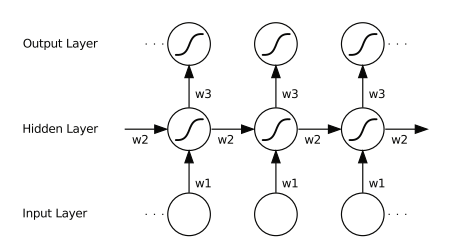
\includegraphics[width=0.6\textwidth]{Figures/lstm/rnn_structure.png}
    \caption{Unfolded Recurrent Network\cite{Graves2012}}
    \label{fig:rnn_structure}
\end{figure}

The activation of each cell is dependent on both it's inputs and the hidden state of the previous time step as illustrated by Equation \ref{eqn:rnn_activation}.\cite{Graves2012}

\begin{equation}
    a_h^t = \sum_{i=1}^I w_{ih}x^t_i + \sum_{h^\prime=1}^H w_{h^\prime h} b_{h^\prime}^{t-1}
    \label{eqn:rnn_activation}
\end{equation}

%What problems exist with them 
RNNs have been shown to produce good results in some sequential task but there application is limited by there difficulty to train, primarily the vanishing/exploding gradient problem. During gradient based training methods repeated multiplication  by values that are not near 1 along long decency chains result in either vanish or explode. A vanishing gradients makes it difficult to know which direction the parameters should move to improve the cost function, while exploding gradients can make learning unstable. Non-gradient based training have been tried although to limited success. \cite{Graves2012, Goodfellow2015}

% LSTM
The Long Short Term Memory (LSTM) architecture solve the vanishing gradient problems by allowing information to be retained for long periods. Originally created by Hochreiter and Schmidhuber in 1997\cite{Hochreiter1997} the LSTM is an RNN style architecture but includes additional paths to control information flow between cells, see Figure \ref{fig:lstm_unit}. Information flowing along the cell state can be modulated by the input and forget gate structures. The final output of the unit is a filtered version of the cell state, the filtering is done based on context from the hidden state.\cite{Olah2015}   % Tensorflow implements the basic cell described by Hochreiter
% Peephole connections \cite{Gers2000}
\begin{figure}[!htb]
    \centering
    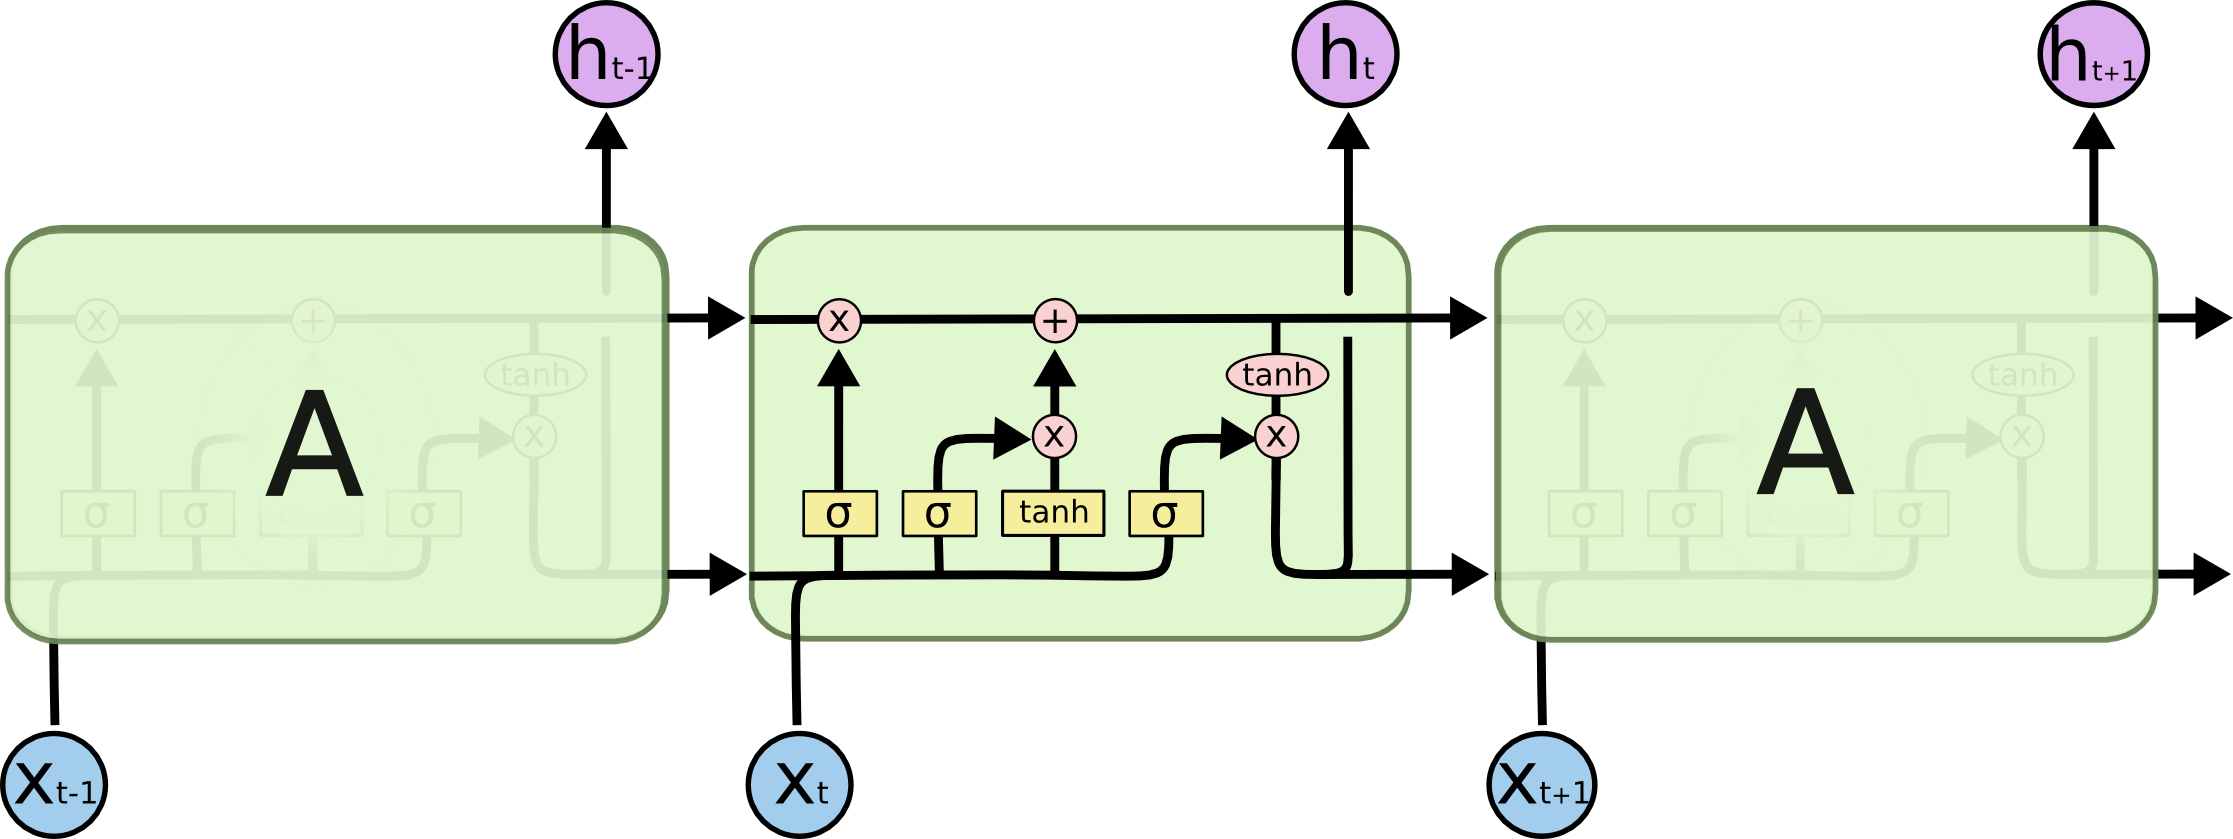
\includegraphics[width=0.7\textwidth]{Figures/lstm/LSTM-chain.png}
    \caption{Diagram of LSTM unit \cite{Olah2015}}
    \label{fig:lstm_unit}
\end{figure}

Like a standard RNN an LSTM contains between each time step and between each layer the network is fully connected. So information must pass through a cell to move forward in time but can mix between cells in the other two dimensions. This gives the model significantly more learning ability but makes understanding its learnt behaviour non trivial.

What are common structures of an LSTM network? <<<NEEDS MORE>>>

%MARG HAR Data
\section{Human Gait Cycle}
A complete gait cycle is defined between two successive Initial Contact (IC) event of the same limb. IC is the point at which any part of the foot contacts the ground. As this is normally the heel this is often refereed to as Heel Strike (HS). The full cycle can be divided into two phases; stance - when the foot is on the ground, and swing when not. The transition from stance to swing is marked by the Toe Off (TO) event and conversely by (HS). The full gait cycle is shown in Figure \ref{fig:gait_cycle}.

\begin{figure}[!htb]
    \centering
    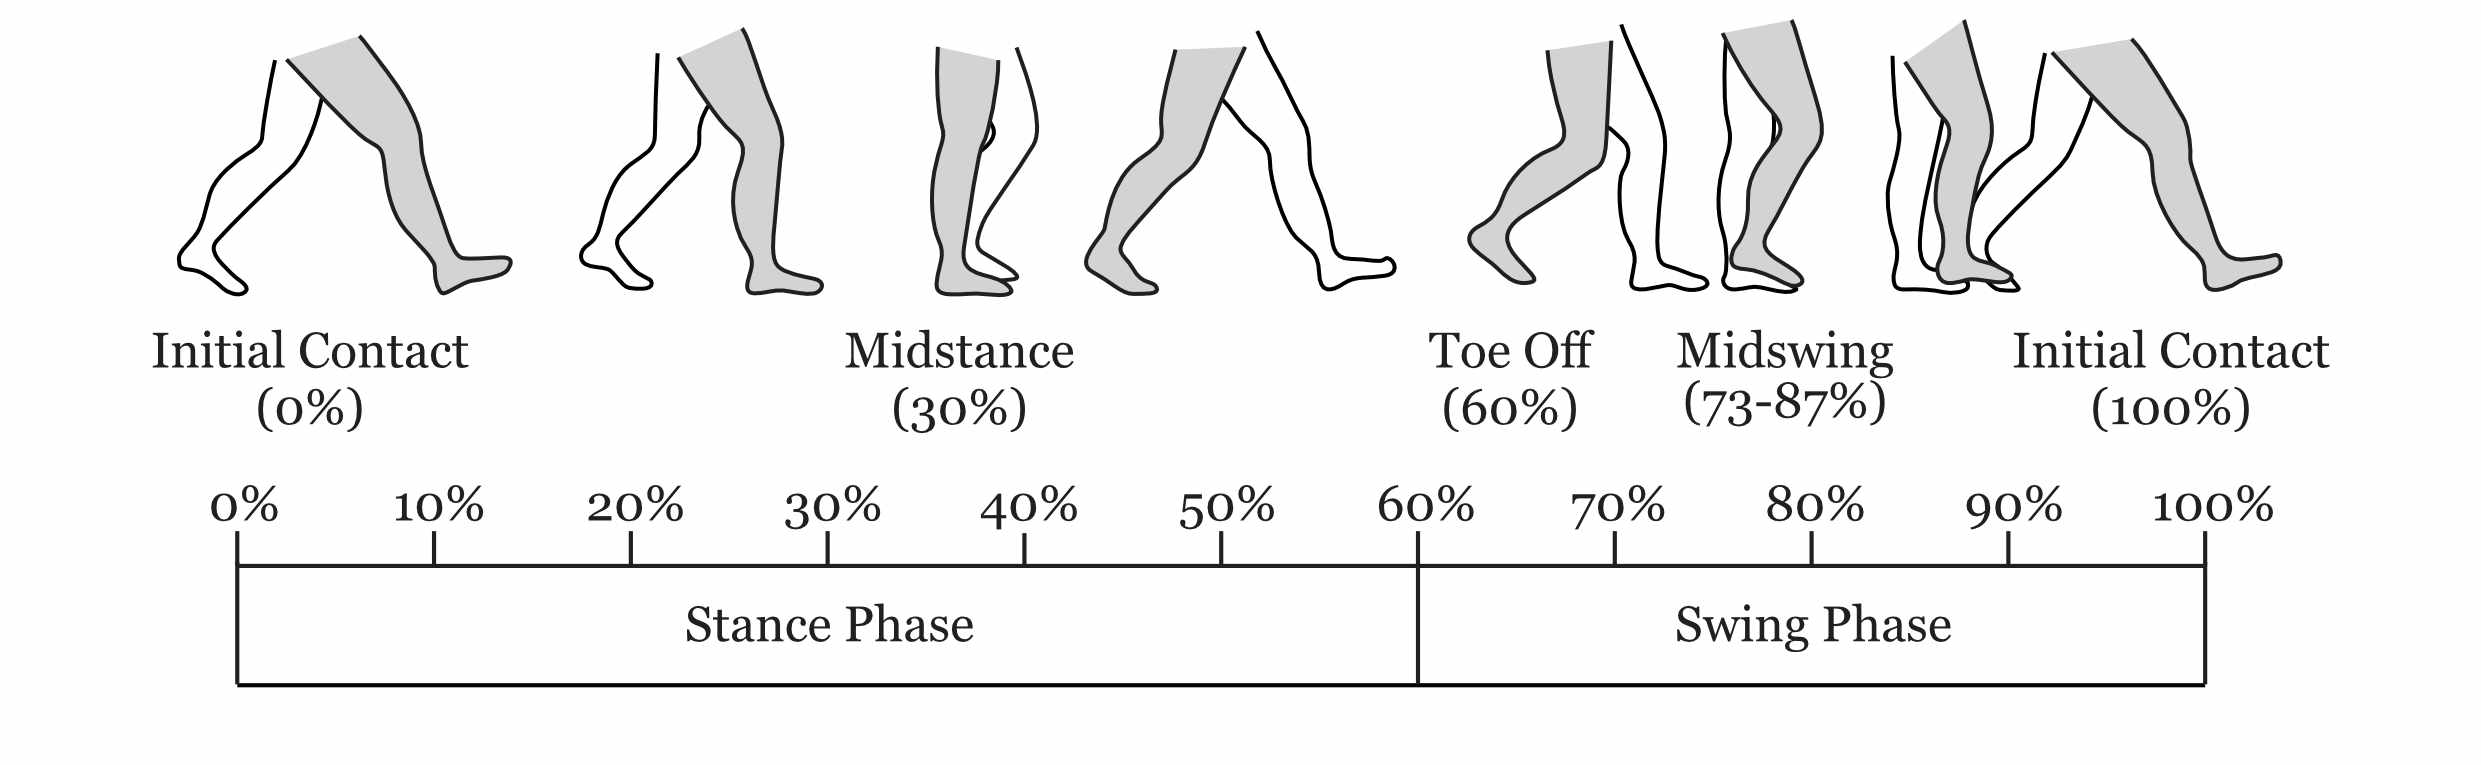
\includegraphics[width=0.8\textwidth]{Figures/Gait_Cycle.jpg}
    \caption{Human Gait Cycle}
    \label{fig:gait_cycle}
\end{figure}

It has been shown that gait cycle can be established from only the shank rotational velocity in the sagittal plane using a technique originally presented by Sabatini et al\cite{Sabatini2005}. The method uses the minima following peak swing angular velocity to approximate heel strike. Toe off as identified as the half way point between the zero crossing and the minima before peak swing. Figure \ref{fig:y-gyro-hs-to} illustrates this.

\begin{figure}[!htb]
    \centering
    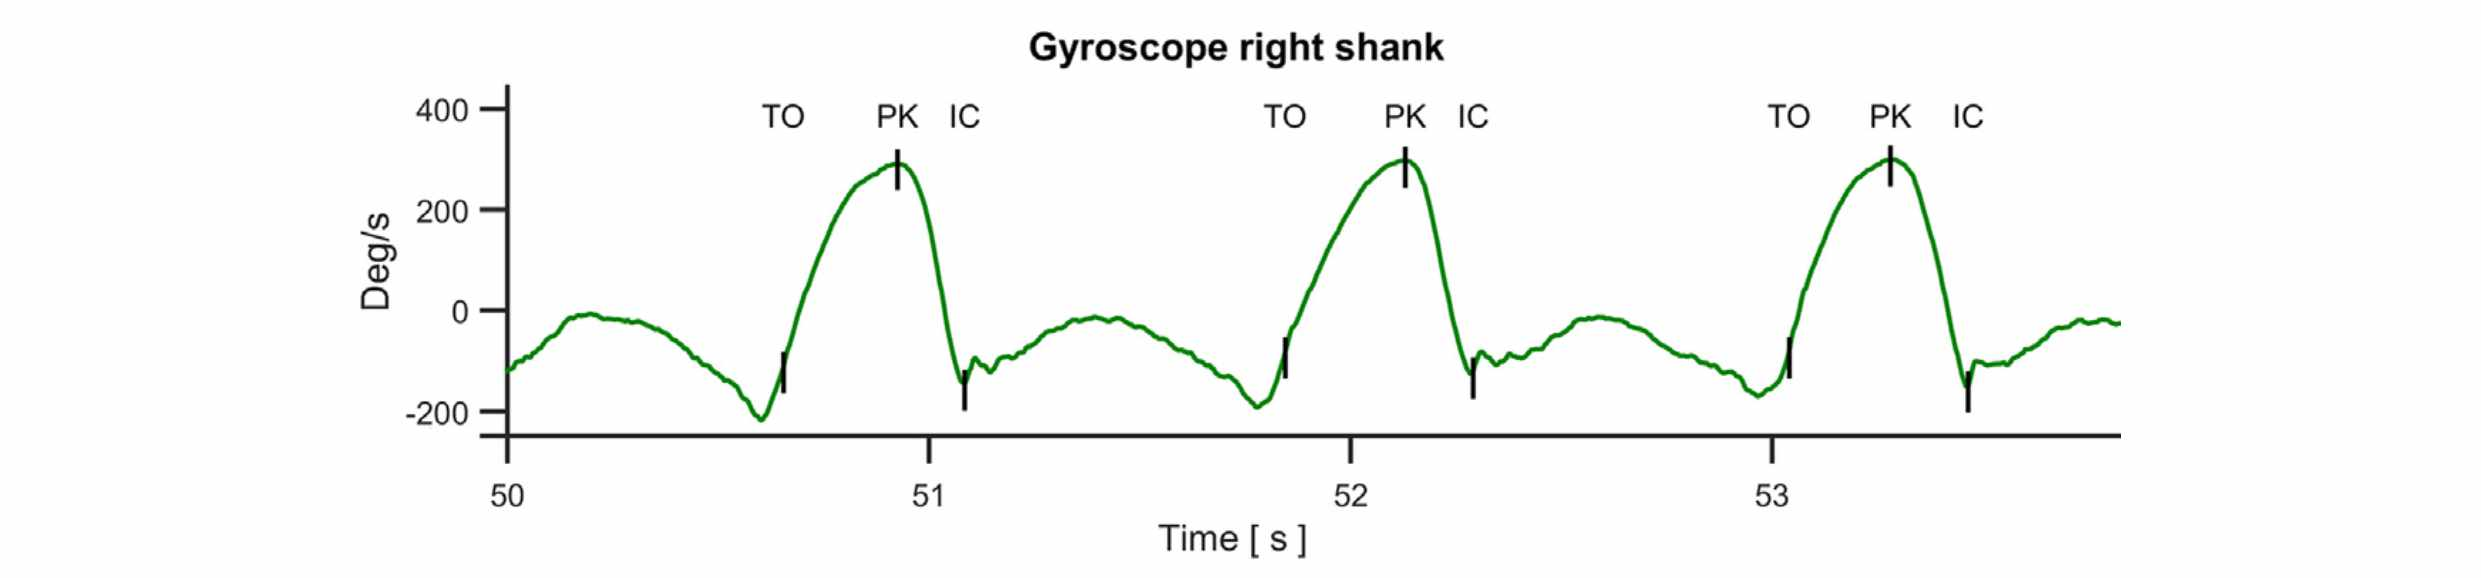
\includegraphics[width=\textwidth]{Figures/gyro_trace_hs.jpg}
    \caption{Gait events extracted from the Sagittal plane gyroscope signal, adapter from \cite{Sabatini2005}}
    \label{fig:y-gyro-hs-to}
\end{figure}

Coley et al noted that the variation in shank sagittal plane rotational velocity occur during different activities. During early stance there is an increase in rotational velocity during stair descent and a decrease in rotational velocity during stair ascent.\cite{Coley2005}


%%%%%%%%%%%%%%%%%%%%%%%%%%%%%%%%%%%%%%%%%%
% \section{Methodology}
% The following section describes the methodology used to investigate the proposed research question.

\section{Data Collection}
In order to investigate machine learning methods a suitable data set is required. This must have the following characteristics, a large number of participants > 20???? with multiple activities captured in a range of environments with transitions between both. <<<NEEDS MORE>>>

No amputee data found - will work can be tested on able bodied participants and amputees used later. Able bodied have less varied gait characteristics than amputee both. <<<NEEDS MORE>>>

% Exsisting data sets
There are several commonly used data sets for able-bodied activity recognition. The OPPORTUNITY activity recognition dataset\cite{roggan2010} contains 18 activity classes for Activities of Daily Living (ADL) such as opening/closing doors and drinking from a cub. Each subject wore seven IMUs and 12 3-axis accelerometers while they preformed the prescribed actions. The UCI-HAD dataset\cite{Anguita2013} recorded subject performing six activities; walking, stair ascent, stair descent, sitting, standing and laying, while recording data from the on board MARG of a waist mounted smart phone. Both of these data sets were recorded in controlled conditions so do not capture any variation in activity that may occur due to the environment. Sztyler and Stuckenschmidt collected data from 15 subjects performing eight activities while wearing six wearable sensors. Recording took place in the same natural environment for each activity, however only steady state activities were capture not the transition between.\cite{Sztyler2017} 

% Aim of data collection
None of the identified data sets achieved all the requirements set out, therefore a new set of data was required. The aim of this data set was to record naturally locomotion in an unstructured environment, capturing both steady state and also the transition between activities across different terrain from a wide range of subjects. Subject were provided with instructions on how to use the sensing equipment and then told to record as they wished. The following activities were selected, Walking (W), Stair Ascent (SA), Stair Descent (SD), Ramp Ascent (RA), Ramp Descent (RD), Stopped (S). These were identified as commonly investigated and required no equipment or skill to perform. 
%This produced a unique self-supervised set of IMU activity data. The self-supervised nature has provided data from a wide range of environments being collected with participants moving at there natural walking speeds with no influence for the researchers.

% Sensor selection and location
Non-invasive wearable sensors, such as Inertial Measurement Units, are an appealing choice for developing such a system. IMU give fast update rate - 100s of Hz, extremely non-invasive (small, minimal mounting constraints), low cost, reasonable accuracy. Widely used, all of the latest generation powered prosthetic knees investigated by Fluit et al contained IMUs \cite{Fluit2020}

% Which sensors did we use and why
A wearable IMU produced by Movesense was used to collect activity data. The device contains a 9 axis MARG (Magnetic, Angular Rate and Gravity) sensor and a Bluetooth radio in a small 10 gram package. The sensor housing contains a snap connectors allowing it to be clipped into attachment hardware and a variety of mounting hardware is available off the shelf. The sensor is user-programmable allowing customised behaviour, in this case it was setup to form a Bluetooth Low Energy (BLE) connection to a smart phone and broadcast the recorded 100Hz MARG sensors data. 

Five sensors were attached to each participant, an the inside of ankle using an elastic Velcro strap, each hip using a clothes/belt clip and the chest using a heart rate strap. The location of the sensors was selected to give a wide covering of body movements while providing secure and non-invasive attachment to minimise discomfort and disruption to natural movement. The sensors are show in Figure \ref{subfig:movesense_sensors}.

% Android app
The data from each sensor was streamed from each sensor at 100Hz to a custom android app. The app contained buttons for real-time annotation of the data. Data recorded from the app could directly sent to the researchers in an anonymous format. A screen shot of the app is shown in figure \ref{subfig:android_app}.<<<NEEDS MORE>>>

\begin{figure}[!hbt]
     \begin{subfigure}[b]{0.49\textwidth}
         \centering
         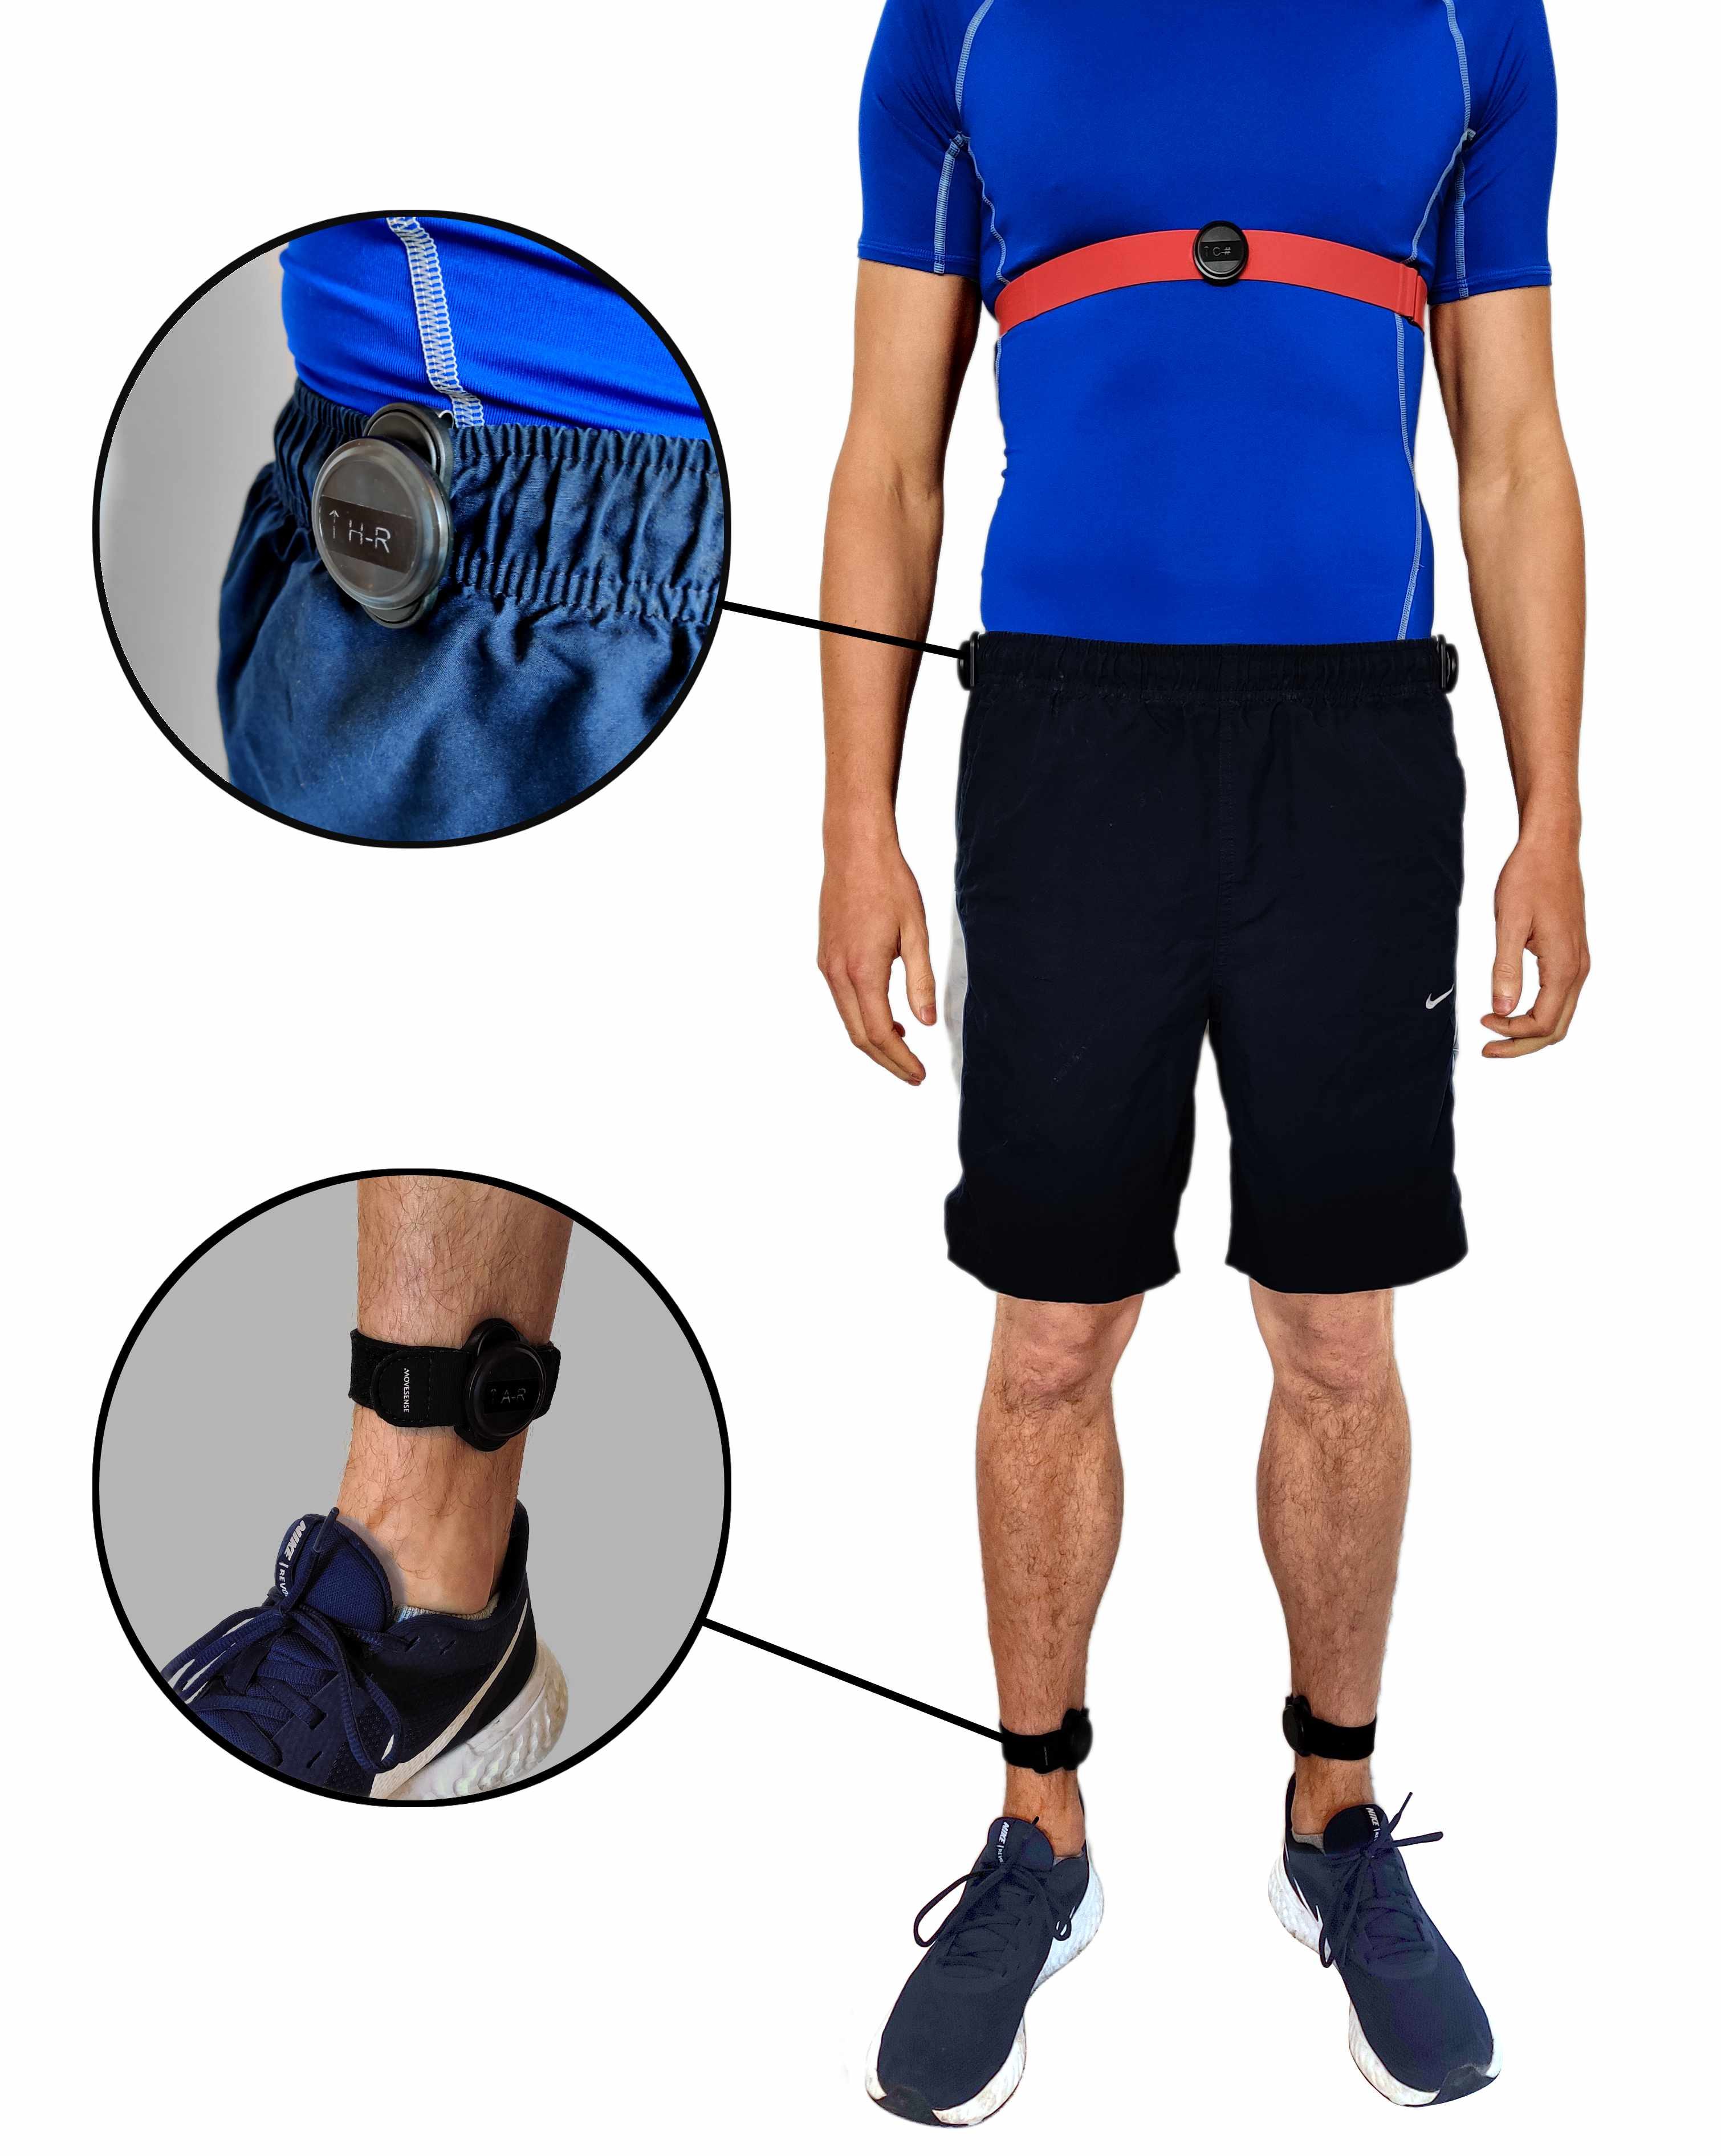
\includegraphics[height=250px]{Figures/movesense/sensor_locations.jpg}
         \captionsetup{justification=centering}
         \caption{Subject wearing the Movesense IMU sensors on both ankles, hips and the chest}
         \label{subfig:movesense_sensors}
     \end{subfigure}
     \hfill
     \begin{subfigure}[b]{0.49\textwidth}
         \centering
         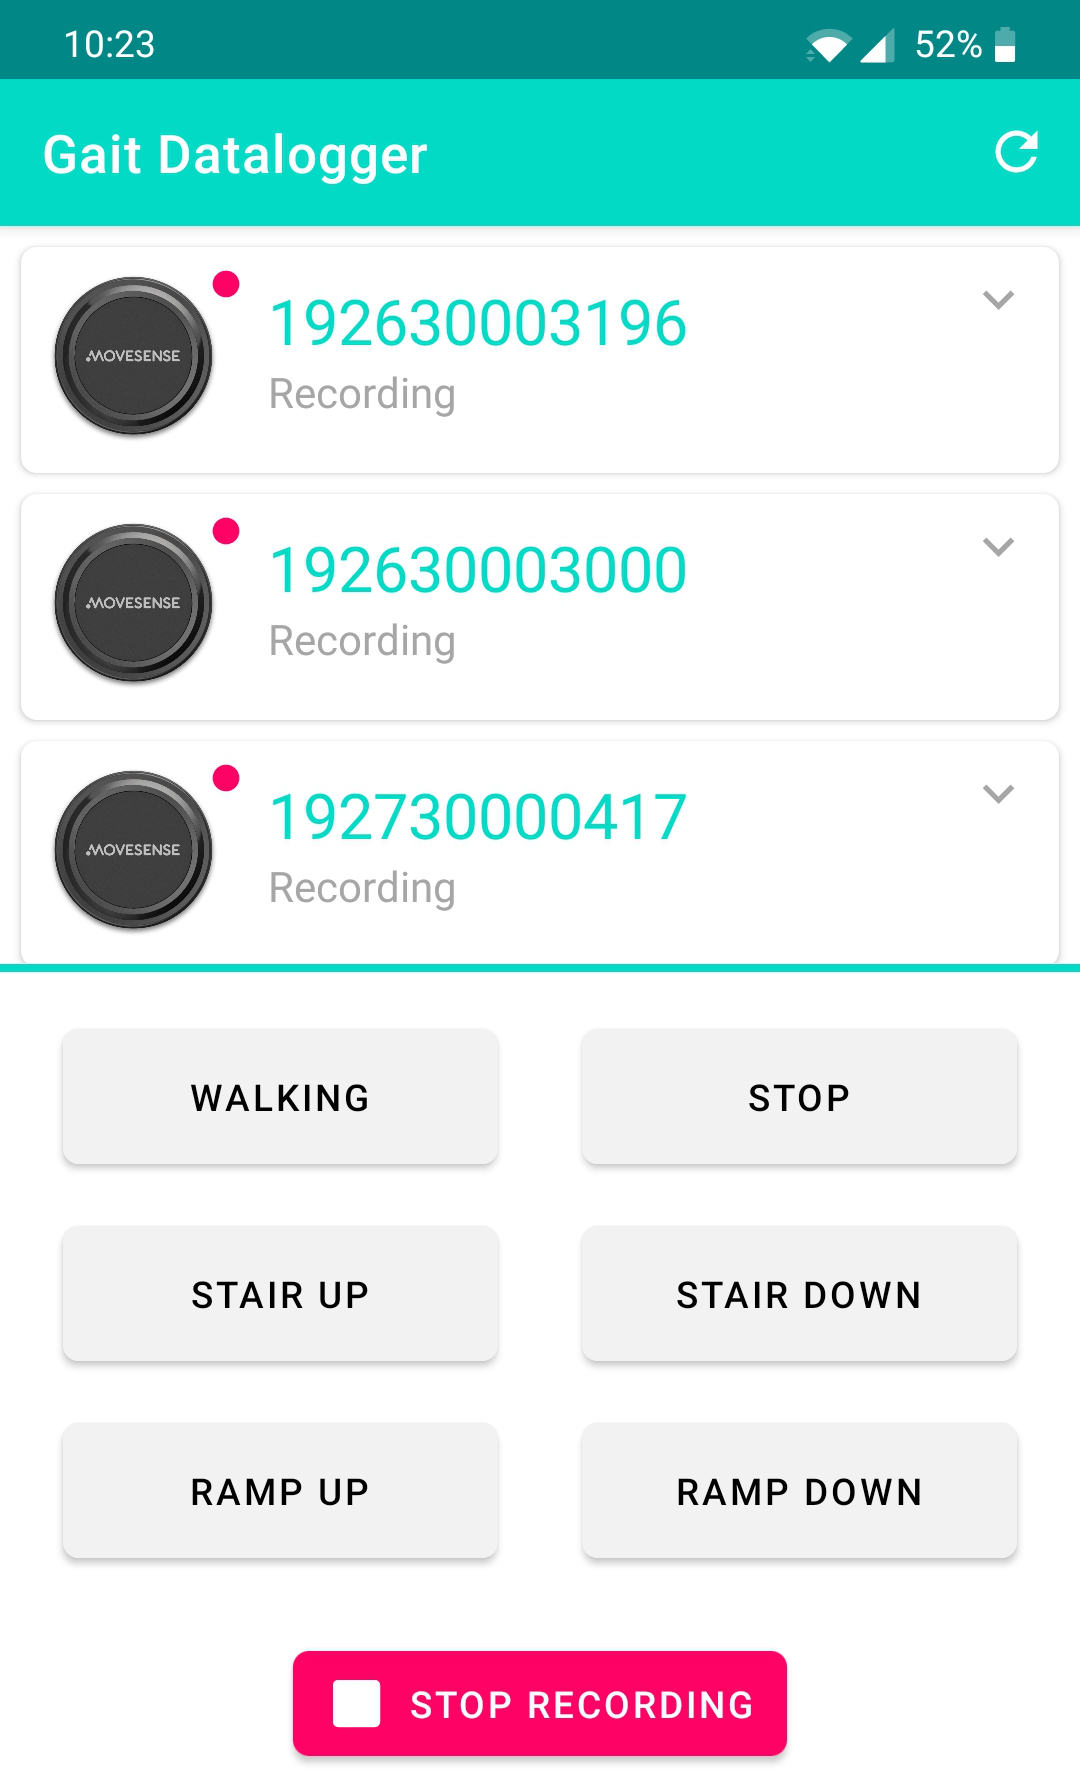
\includegraphics[height=250px]{Figures/movesense/app_recording_short.jpg}
         \captionsetup{justification=centering}
         \caption{Custom Android app used to record and annotate the sensor data}
         \label{subfig:android_app}
     \end{subfigure}
    \caption{Data recording setup}
    \label{fig:imu_sensors and app}
\end{figure}

% Participant instructions
Twenty-two Participants of a wide variety of age, gender and physique were chosen to give a broad data set. Participants were instructed to walk around a varied environment with the sensor on, and label their activity as they went. No further instructions on how the activities should be conducted were provided. <<<NEEDS MORE>>>

% How much data did we collect
A total of 268 minutes of data was collected that included 1170 transitions between activities. Table \ref{tab:data_collected_summary} contains a summary of the data collected.<<<NEEDS MORE>>>

% Dataset Statistics
\begin{table}[!hbt]
    \centering
    \caption{Quantity of data collected for each activity}
    \label{tab:data_collected_summary}
    \begin{tabular}{cccc}
        \textbf{Activity} & \textbf{Samples} & \textbf{Time (minutes)} & \textbf{Number of Steps} \\
         \hline
         Walking & 1075211 & 179 & 9438 \\
         Stair Ascent & 139922 & 23 & 1286 \\
         Stair Descent & 122379 & 20 & 1280 \\ 
         Ramp Ascent & 73328 & 12 & 656 \\
         Ramp Descent & 79436 & 13 & 754 \\
         Stop & 121027 & 20 & - \\
         \hline
         \textbf{Total} & 1611303 & 268 & 13414
    \end{tabular}
\end{table}

% Data post-processing
To convert the raw saved data to a form that Tensorflow could understand from using a processing pipeline was developed in Matlab 2019b. The pipeline consisted of decoding, re-sampling, normalisation, and saving. The data is saved raw from the sensor so needed to be converted from compressed hexadecimal fixed point form to a floating-point representation. The data was then re-sampled to compensate for the difference between the internal sensor clock, the android smartphone clock was used as a common reference for this adjustment. The data was normalised so that for each recording every individual sensor channel had a standard deviation of one and a mean of zero.

% Data axis system
The following axis system will be used when presenting and analysing the results. The axes uses a right hand front left up convention. $x$ is forward towards the front of the foot, $y$ toward the left of the body and $z$ upwards. Figure \ref{fig:data_axis} illustrates this.<<<NEEDS MORE>>>
% \begin{wrapfigure}{l}{0.5\textwidth}
\begin{figure}[!htb]
    \centering
    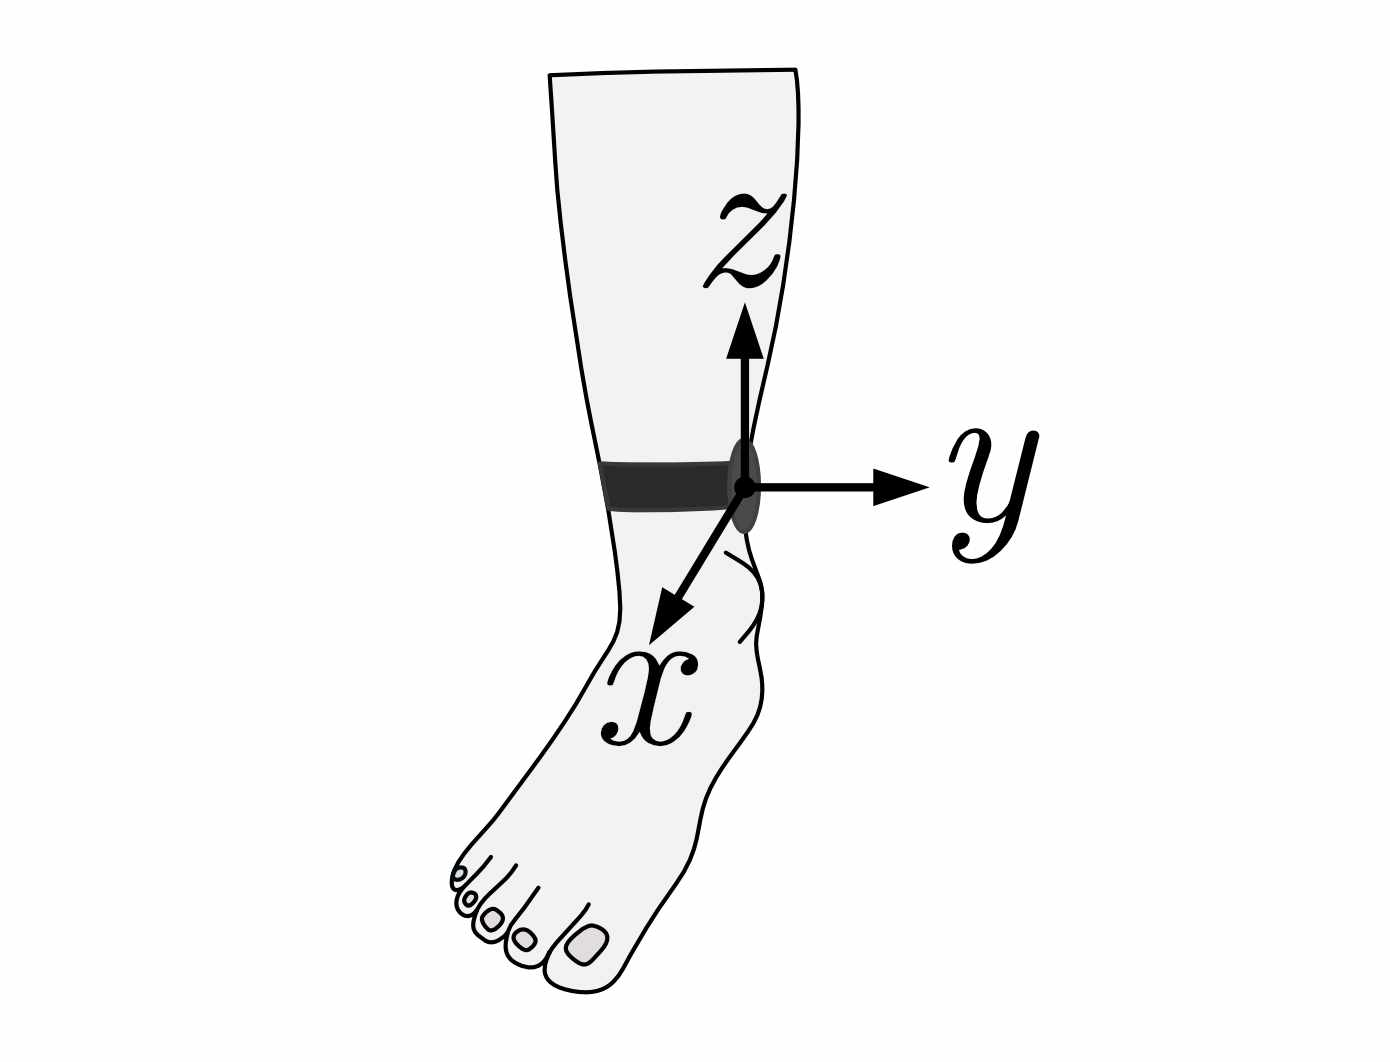
\includegraphics[width=0.4\textwidth]{Figures/ankle_axis.jpg}
    \caption{Right ankle data axis}
    \label{fig:data_axis}
\end{figure}
% \end{wrapfigure}

For the simplicity of data analysis within this paper the start of the gait cycle will be defined as the peak swing velocity as measured in the gyroscope y axis. Gait cycle is given as percentage of the time period of the each gait cycle, peak swing to peak swing.<<<NEEDS MORE>>>

%%%%%%%%%%%%%%%%%%%%%%%%%%%%%%%%%%%%%%%%%%
\section{Machine Learning Methods}
Within this section the methodology for the machine learning models and methods that will be used to answer the proposed research questions are provided. First the training procedure will be discussed, this will be followed by the simplified model used to investigate the networks internal learnt behaviour. Finally the methods for investigating how hyper-parameters of an LSTM network performance are discussed.

Training - The adam optimisation algorithm was used, a popular algorithm for problems with large data-sets and or parameters[1]. The training was undertaken using GPU acceleration with models defined using the Tensorflow 2.1.0 and Keras. Initial model weights were set using a Golorot Uniform initialiser. A class weight input was used to bias the training as a balance for in-balanced data labels. A mini batch size of 2000 was used with early stopping based on validation data cross entropy loss. Dropout of "0.5, which seems to be close to optimal for a wide range of networks and tasks.”\cite{Srivastava2014}<<<NEEDS MORE>>>

A sliding data window will be used to divide the data. An offset of 2 samples will be used as the overlap. The offset was set empirically to give the model a wide range of data from any window position without slowing down training from an unnecessarily large data set. The label for each widow was set as the recorded ground truth at the end of the window, these are provided to the network in a one-hot encoding.<<<NEEDS MORE>>>

The training data set is divided into two groups a test and training. The test set is a variation on the Leave One Out Cross Validation (LOOXV), to reduce computational time for each mode four/five participants are excluded from the training process to be used as unseen data for accessing the model generalisation performance. The training set contains the remaining participants. The training set was reduced so that no label class contains more than 50\% greater labels than any another. For each model, the training data 30\% was retained as validation the remaining 70\% used for training. The data was split randomly but care was taken to ensure the balance of each label type was maintained. The training process is repeated 5 time independently so each participant is excluded once from the training data set. By combining the results from each model an assessment of generalisation can be performed.

% Simplified model
<TK>In literature most LSTM model are structured as in Figure \ref{fig:full_lstm_model}. The raw sensor data is fed as an input vector into the first LSTM layer of n units. The hidden state vector from this layer is then fed into subsequent LSTM layers. The last output of the final LSTM layer is passed into a dense classification layer. Some authors have used a fully connected final layer using the output from every cell, termed later fusion, although no justification for this architecture has been given.

\begin{figure}[!htb]
    \centering
    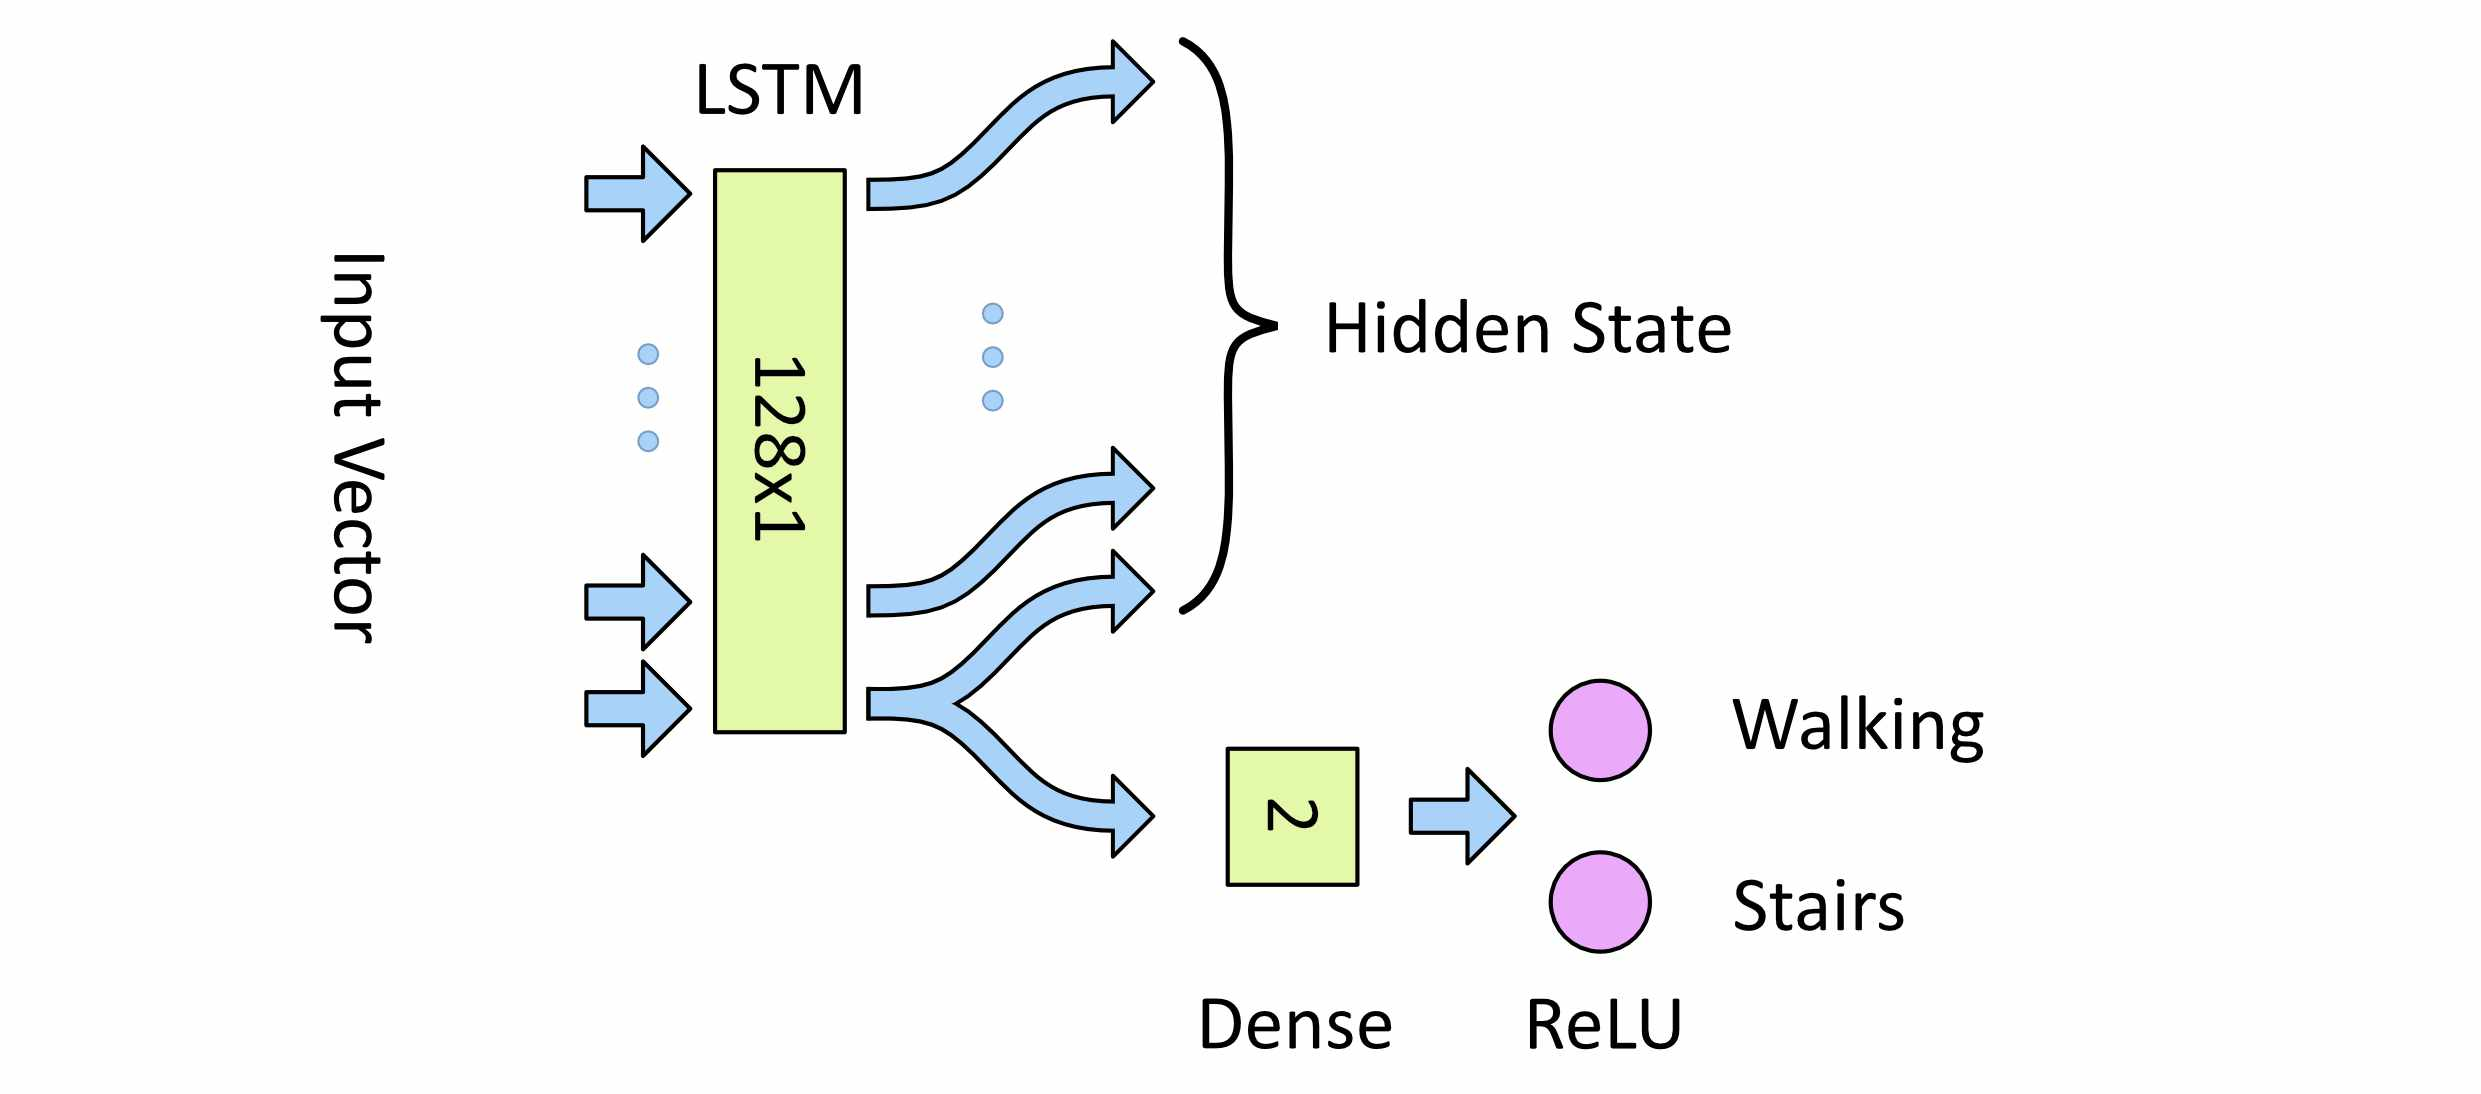
\includegraphics[width=0.8\textwidth]{Figures/lstm/Simplified_Network.jpg}
    \caption{Illustration of simplified model}
    \label{fig:full_lstm_model}
\end{figure}

Looking to understand what features the model is learning. Full model too complex to interpret due to many fully connected steps making following the path of information extremely challenging. If only a single path is provided for information to flow it would be straight forward to determine which parts of an input signal produce what behaviour. To achieve this a simplified model should be used.

% Simplified model - plotting of hidden state
Single unit single layer network with final hidden state passed to dense layer before a Relu activation and classifier. Logits and Relu have been used to ensure no scaling occurs across the network. The simplified model provides only 1 path form information to flow, therefore should be easier to establish which parts of the input signal extracted to classify. The hidden state of the model can be extracted by copying the LSTM weights and biases from the trained model to a new model which outputs just the full sequence of hidden state.

% How are we simplifying the classification problem so the basic model can solve it
Justification for simplifying the problem. The simple model is not complex enough to solve the full problem, as such in order to get a reasonable classification accuracy the problem needs to be simplified. This simplification can be done either through reducing the number of classes or only training the network to understand certain classes. How are we simplifying the problem? A combination of both will be used, training the model to classify the three most prevalent activities in the data set, W, SA, SD, in different combinations. For example a walking class and a stair class (SA and SD). Why are we only looking at the ankle sensor? <<<NEEDS MORE>>>

% Analysis methods
To observe the change in information level within network the hidden state value will be used. This will be plotted such that patterns in output for different activities can be seen. To achieve this multiple windows of data will be plotted over top each other all with the same starting point. To account for variation in gait cadence throughout the data set the x axis will be plotted as percentage of gait cycle. Each different activity will be plotted independently. The information gained from these observations will be tested against performance of the full model.

% Full Model
To solve the full problem a more complex model will be used, using variations on the architecture presented by Murad et al discussed in \ref{sec:related_works}. The effect of hyper-parameters on it's performance will be evaluated by para-metrically sweeping those appropriate. This will allow ideas and observations established from the simplified model to be tested to see if the knowledge is transferable to more complex examples.

For models with fully connected layers the hidden state becomes too convoluted to interpret directly. Classification performance will be analysed using percentage accuracy, of the validation data for model performance, and using the novel unseen data as a metric for it's generality. Confusion matrices can be used to establish how well the model does as separating output classes from one another.

Which hyper-parameters are we going to investigate? Window size, LSTM units, layers, inputs (number of axis, number of sensors), number of participants <<<Needs More>>>

%%%%%%%%%%%%%%%%%%%%%%%%%%%%%%%%%%%%%%%%%%
\section{Results and Analysis}
In this section the results of the analysis conducted are presented.<<<NEEDS MORE>>>

%%%%%%%%%%%%%%%%%%%%%%%%%%%%%%%%%%%%%%%%%%
\subsection{Individual Gait Trends}
In order to gauge how different each subject gait is the trends for different activities for each axis were produced. The angular velocity around y and the acceleration in x showed the greatest variation between subjects. Below the trends for these axis for two subject is shown. Figure \ref{fig:imu_gait_trends} shows the mean and standard deviation for three difference activities (W, SA, SD) for two individual subjects. The solid line represents the mean of n gait cycles, and the shaded area the standard deviation. Figures \ref{subfig:x_accel_subj_4} and \ref{subfig:x_accel_subj_16} show the acceleration in the x axis for participants four and sixteen respectively. Figure \ref{subfig:x_gyro_subj_4} and \ref{subfig:x_gyro_subj_16} show the angular velocity in the y axis for the same participants.

\begin{figure}[!htb]
     \centering
     \begin{subfigure}[b]{0.49\textwidth}
         \centering
         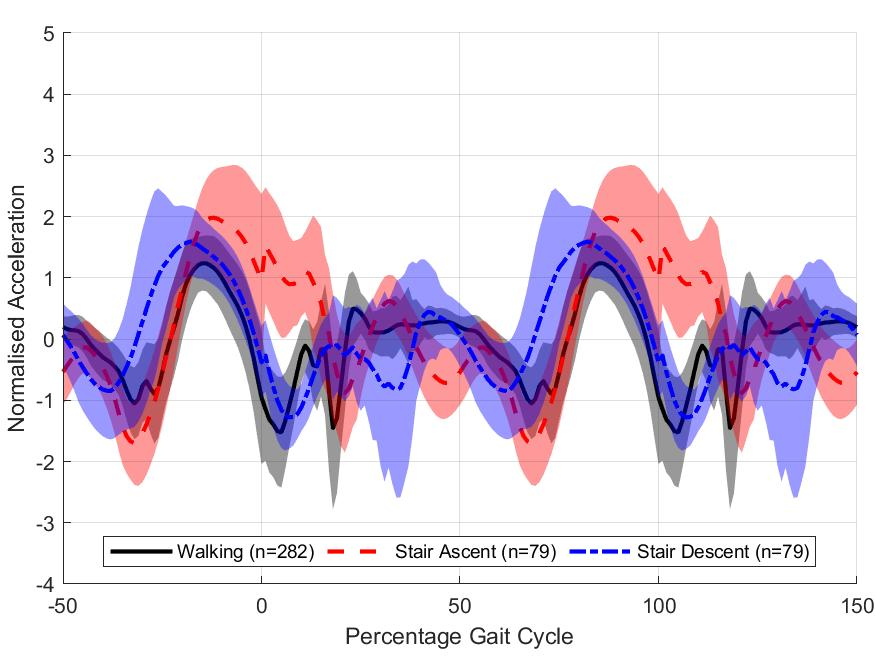
\includegraphics[width=\textwidth]{Figures/gait_trends/accel_x_trend_Participant_04.jpg}
         \caption{Subject 4 - Acceleration in x}
         \label{subfig:x_accel_subj_4}
     \end{subfigure}
     \hfill
     \begin{subfigure}[b]{0.49\textwidth}
         \centering
         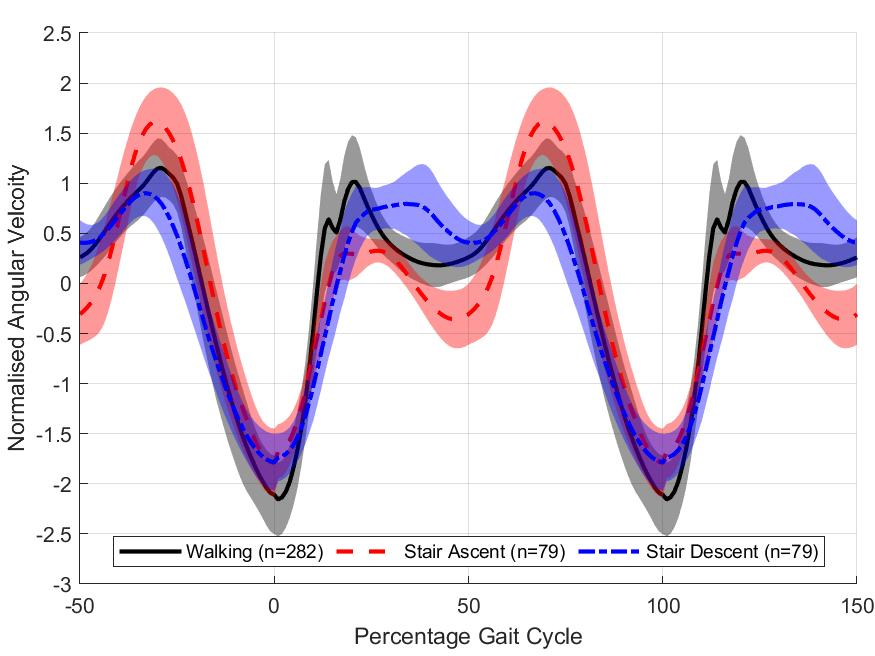
\includegraphics[width=\textwidth]{Figures/gait_trends/gyro_y_trend_Participant_04.jpg}
         \caption{Subject 4 - Shank angular velocity about y}
         \label{subfig:x_gyro_subj_4}
     \end{subfigure}
     \vskip\baselineskip
     \begin{subfigure}[b]{0.49\textwidth}
         \centering
         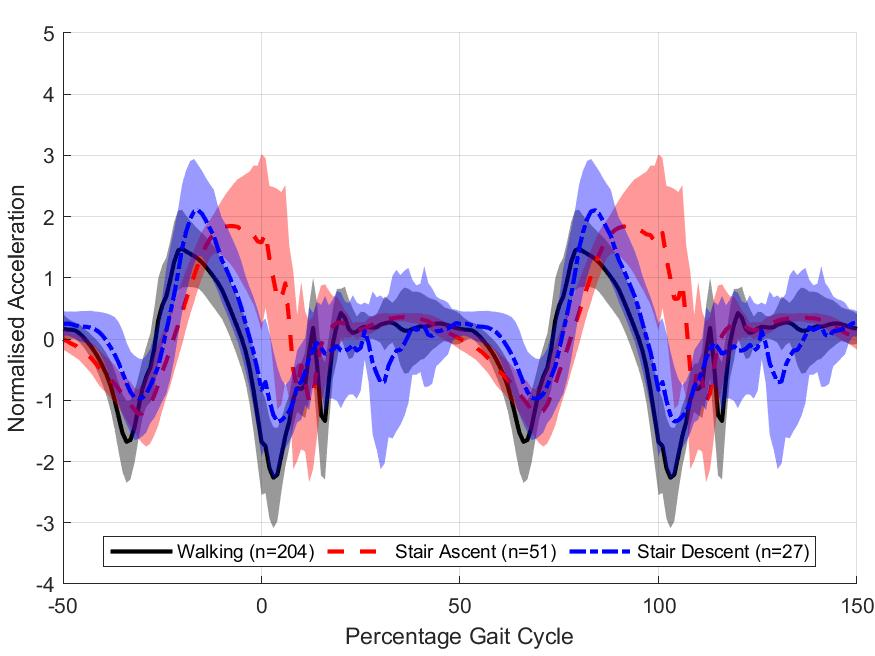
\includegraphics[width=\textwidth]{Figures/gait_trends/accel_x_trend_Participant_16.jpg}
         \caption{Subject 16 - Shank acceleration in x}
         \label{subfig:x_accel_subj_16}
     \end{subfigure}
     \hfill
     \begin{subfigure}[b]{0.49\textwidth}
         \centering
         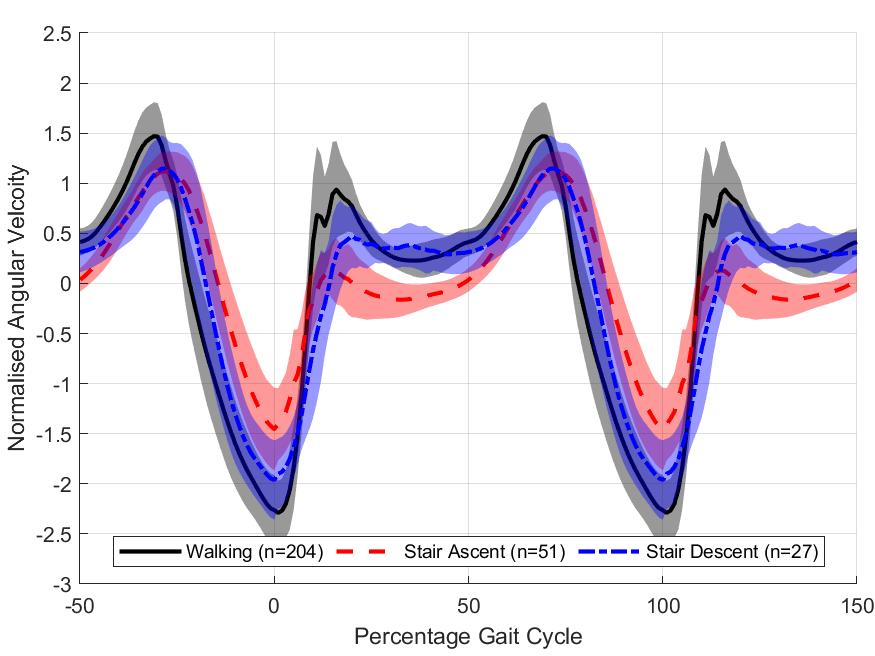
\includegraphics[width=\textwidth]{Figures/gait_trends/gyro_y_trend_Participant_16.jpg}
         \caption{Subject 16 - Shank angular velocity about y axis}
         \label{subfig:x_gyro_subj_16}
     \end{subfigure}
    \caption{Gait trends of two subject for 3 different activities. The solid lines show the mean value for n steps, the shaded area shows the standard deviation. Black solid - Walking, Red dashed - Stair Ascent, Blue dot dash - Stair Descent}
    \label{fig:imu_gait_trends}
\end{figure}

From Figure \ref{fig:imu_gait_trends} the differences between the two chosen participants can be seen. The x acceleration signal is very noisy, with large standard deviation particularly around heel strike, ~20\% gait cycle. For stair ascent there is a delayed peak acceleration with stair descent and walking having very similar shapes.

As explained previously 0\% gait cycle corresponds with the peak y axis shank angular velocity. The maxima following this is a pseudo point for heel strike and the maxima prior for toe off. As expected stair descent results in a large early stance angular velocity and stair ascent a decrease. The difference in peak angular velocity between participants likely a result of climbing stairs at a slower cadence.

The graphs are largely similar, this holds true for the other subjects not shown here, with early stance having the greatest difference between participants for both acceleration and angular velocity. This appears to be the area with greatest information about locomotion mode so may cause issues when generalising.

%%%%%%%%%%%%%%%%%%%%%%%%%%%%%%%%%%%%%%%%%%
\subsection{Simplified Model}
Within this section the results of the simplified LSTM model are presented. Four different combinations of output class for the activities Walking, Stair Ascent and Stair Descent, were tested as well as four different combinations of input sensor, Y Gyroscope, X Accelerometer, Y Gyro \% X Accel and the full 6 axis IMU. The y gyroscope and x accelerometer were selected as from the previous analysis they showed the greatest variation between subjects.

Table \ref{tab:simplified_model_perfomances} presents the classification accuracies of each input and class combination. For each model classification accuracy was recorded for the validation data and a set of unseen test data from excluded participants. It can be seen that all the models performed equally well for both validation and test data sets. Given the simplicity of the models this suggests that an LSTM is capable of separating the activities from only prominent features.

The models struggled to separate stair descent from the other two activities and, apart from with the 6 axis IMU, most accurately classified stair ascent. From the gait trends this is likely because stair ascent is the most different of the three. All achieved there lowest performance when attempting the hardest task of classifying all three activities individually. An input of the X accelerometer on it's own performed most accurately, even compared to models with multiple input sensors channels. When using only the Y Gyroscope it wasn't possible to separate three activities independently.

\begin{table}[!hbt]
    \centering
    \caption{Summary of simplified model performance}
    \label{tab:simplified_model_perfomances}
    \begin{tabular}{cccc}
        \textbf{Model Classes} & \textbf{Sensor} & \textbf{Validation Accuracy} & \textbf{Test Accuracy}\\
        \hline
        W, SA+SD & Y Gyroscope & 71.6\% & 86.0\% \\
        SA, W+SD & Y Gyroscope & 82.7\% & 83.7\% \\
        SD, W+SA & Y Gyroscope & 57.9\% & 65.6\% \\
        *W, SA, SD & Y Gyroscope & - & - \\
        W, SA+SD & X Accelerometer & 86.6\% & 89.2\% \\
        SA, W+SD & X Accelerometer & 88.6\% & 87.1\% \\
        SD, W+SA & X Accelerometer & 78.4\% & 81.9\% \\
        W, SA, SD & X Accelerometer & 71.9\% & 72.4\%\\
        W, SA+SD & X Accel \& y Gyro & 59.3\% & 48.8\% \\
        SA, W+SD & X Accel \& y Gyro & 71.2\% & 67.1\% \\
        SD, W+SA & X Accel \& y Gyro & 75.1\% & 80.8\% \\
        W, SA, SD & X Accel \& y Gyro & 58.6\% & 66.2\%\\
        W, SA+SD & 6 axis IMU & 82.0\% & 83.3\% \\
        SA, W+SD & 6 axis IMU & 74.2\% & 71.8\% \\
        SD, W+SA & 6 axis IMU & 55.3\% & 63.3\% \\
        W, SA, SD & 6 axis IMU & 48.0\% & 50.7\%\\
        \multicolumn{4}{l}{\footnotesize{* Unable to train a model that could classify this set of classes}}
    \end{tabular}
\end{table}

\subsection{Hidden State}
Figures \ref{fig:hidden-state-gyro-y-w_v_sa-sd} and \ref{fig:hidden-state-accel-x-w_v_sa-sd} show the trend in hidden state value for a simplified model. In Figure \ref{fig:hidden-state-gyro-y-w_v_sa-sd} the model is classifying stair ascent from a combined class of stair descent and walking. For figure \ref{fig:hidden-state-accel-x-w_v_sa-sd} the model is classifying walking from stairs (ascent and descent). Each of the activities is plotted in a different color, blue solid for walking, green dashed for stair ascent and orange dot dash for stair descent. The five plots each show the hidden state for each timestep with each window starting at the same percentage offset from the beginning of the gait cycle. The x-axis has units of percentage gait cycle, the Y-axis is the dimensionless output of the hidden state. Figure \ref{fig:hidden-state-gyro-y-w_v_sa-sd} has an input of the Y axis gyroscope and \ref{fig:hidden-state-accel-x-w_v_sa-sd} the x accelerometer.

\begin{figure}[!hbt]
     \centering
     \begin{subfigure}[b]{0.32\textwidth}
         \centering
         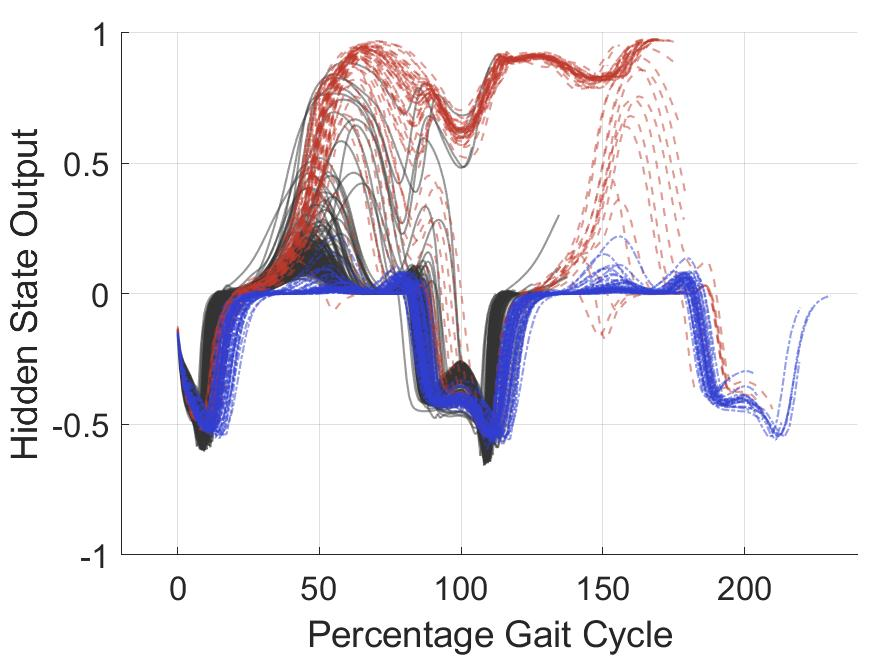
\includegraphics[width=\textwidth]{Figures/results/hidden_state/gyro_y_sa_v_w-sd/0_Participant_04.jpg}
         \caption{0\%}
         \label{subfig:gyro_y_w_v_sa_sd_0}
     \end{subfigure}
     \hfill
     \begin{subfigure}[b]{0.32\textwidth}
         \centering
         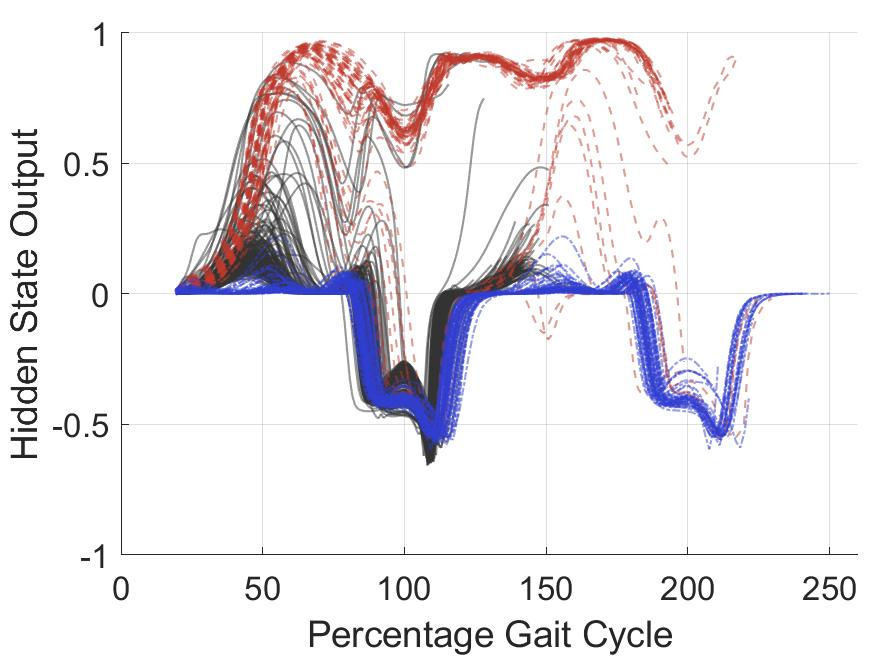
\includegraphics[width=\textwidth]{Figures/results/hidden_state/gyro_y_sa_v_w-sd/20_Participant_04.jpg}
         \caption{20\%}
         \label{subfig:gyro_y_w_v_sa_sd_20}
     \end{subfigure}
     \hfill
     \begin{subfigure}[b]{0.32\textwidth}
         \centering
         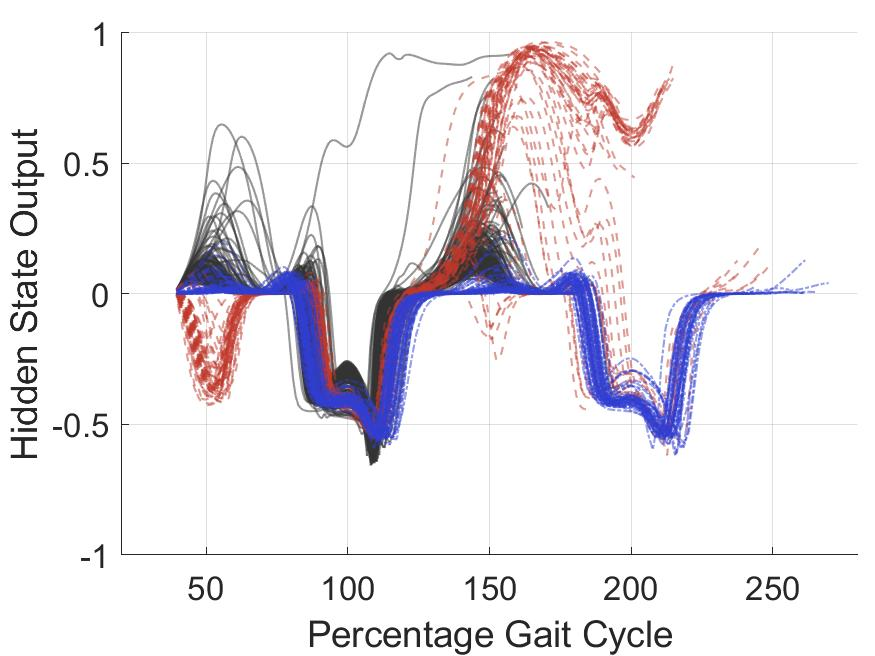
\includegraphics[width=\textwidth]{Figures/results/hidden_state/gyro_y_sa_v_w-sd/40_Participant_04.jpg}
         \caption{40\%}
         \label{subfig:gyro_y_w_v_sa_sd_40}
     \end{subfigure}
     \vskip\baselineskip
     \begin{subfigure}[b]{0.32\textwidth}
         \centering
         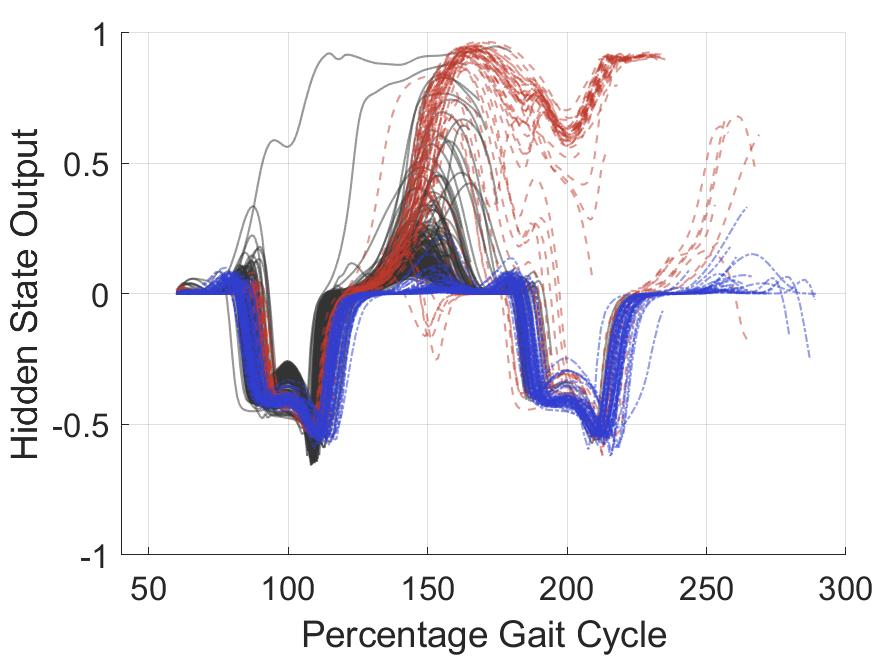
\includegraphics[width=\textwidth]{Figures/results/hidden_state/gyro_y_sa_v_w-sd/60_Participant_04.jpg}
         \caption{60\%}
         \label{subfig:gyro_y_w_v_sa_sd_60}
     \end{subfigure}
     \hspace{0.5em}
     \begin{subfigure}[b]{0.32\textwidth}
         \centering
         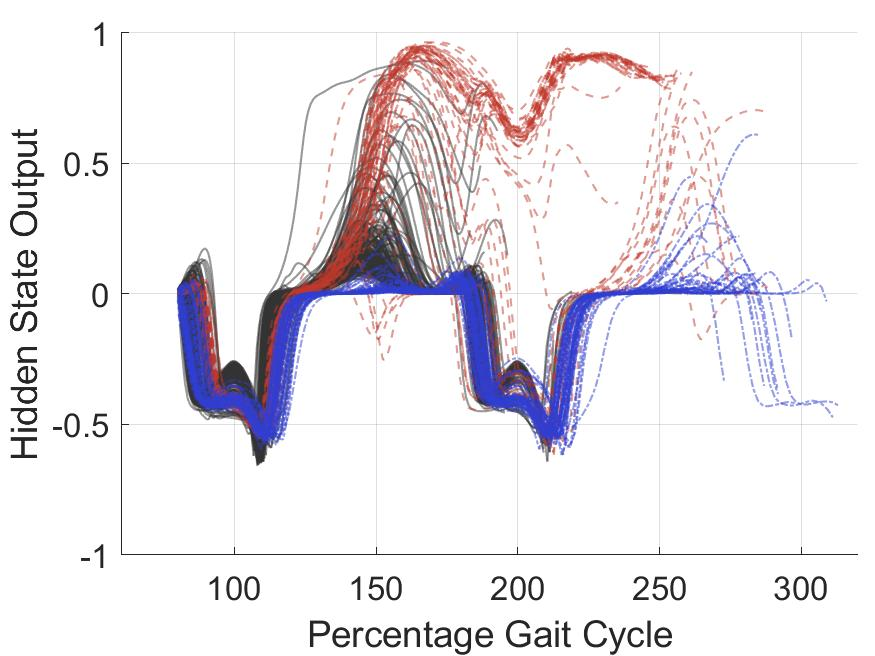
\includegraphics[width=\textwidth]{Figures/results/hidden_state/gyro_y_sa_v_w-sd/80_Participant_04.jpg}
         \caption{80\%}
         \label{subfig:gyro_y_w_v_sa_sd_80}
     \end{subfigure}
    \caption{Hidden state of single unit LSTM model with x axis accelerometer as it's input. The model output classifies stair ascent from walking and stair descent. walking (blue), stair ascent (green) and stair descent (orange)}
    \label{fig:hidden-state-gyro-y-w_v_sa-sd}
\end{figure}

\begin{figure}[!hbt]
     \centering
     \begin{subfigure}[b]{0.32\textwidth}
         \centering
         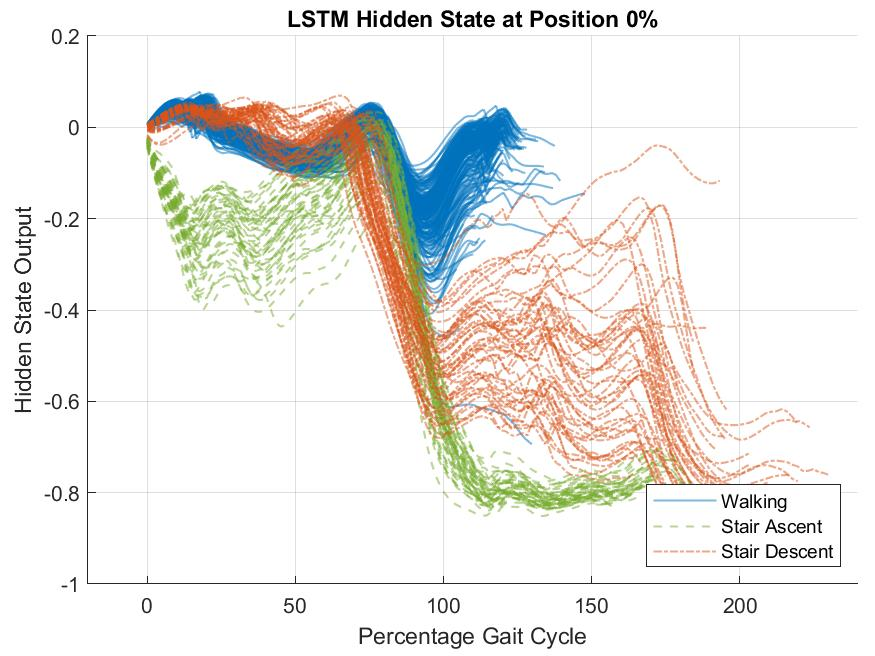
\includegraphics[width=\textwidth]{Figures/results/hidden_state/accel_x_w_v_sa-sd/0_Participant_04.jpg}
         \caption{0\%}
         \label{subfig:a}
     \end{subfigure}
     \hfill
     \begin{subfigure}[b]{0.32\textwidth}
         \centering
         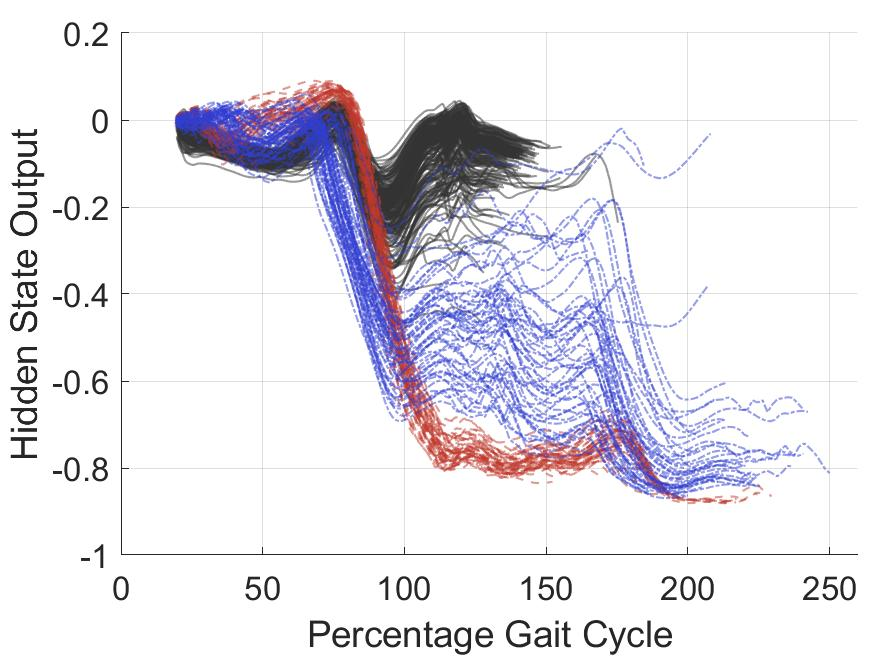
\includegraphics[width=\textwidth]{Figures/results/hidden_state/accel_x_w_v_sa-sd/20_Participant_04.jpg}
         \caption{20\%}
         \label{subfig:b}
     \end{subfigure}
     \hfill
     \begin{subfigure}[b]{0.32\textwidth}
         \centering
         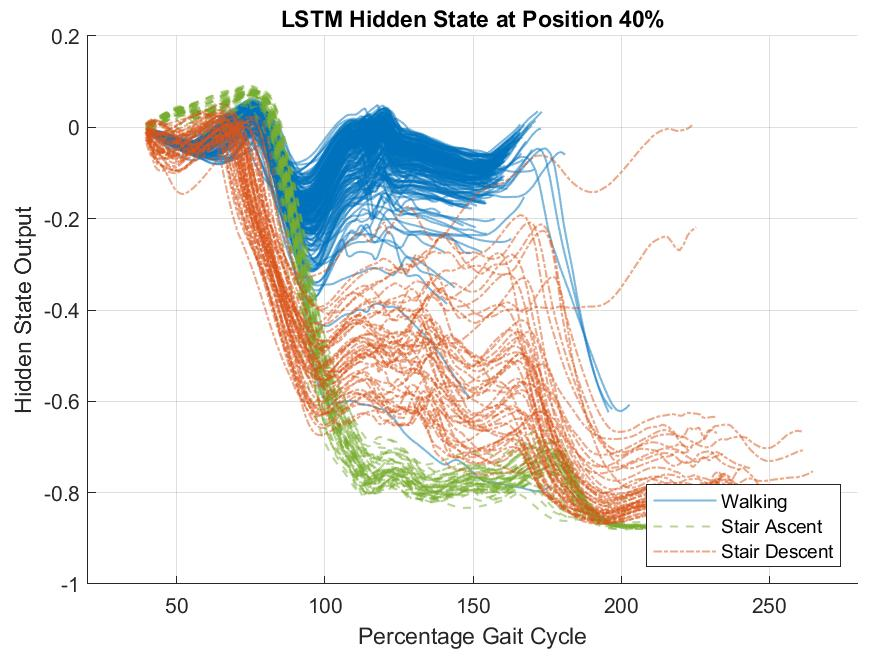
\includegraphics[width=\textwidth]{Figures/results/hidden_state/accel_x_w_v_sa-sd/40_Participant_04.jpg}
         \caption{40\%}
         \label{subfig:c}
     \end{subfigure}
     \vskip\baselineskip
     \begin{subfigure}[b]{0.32\textwidth}
         \centering
         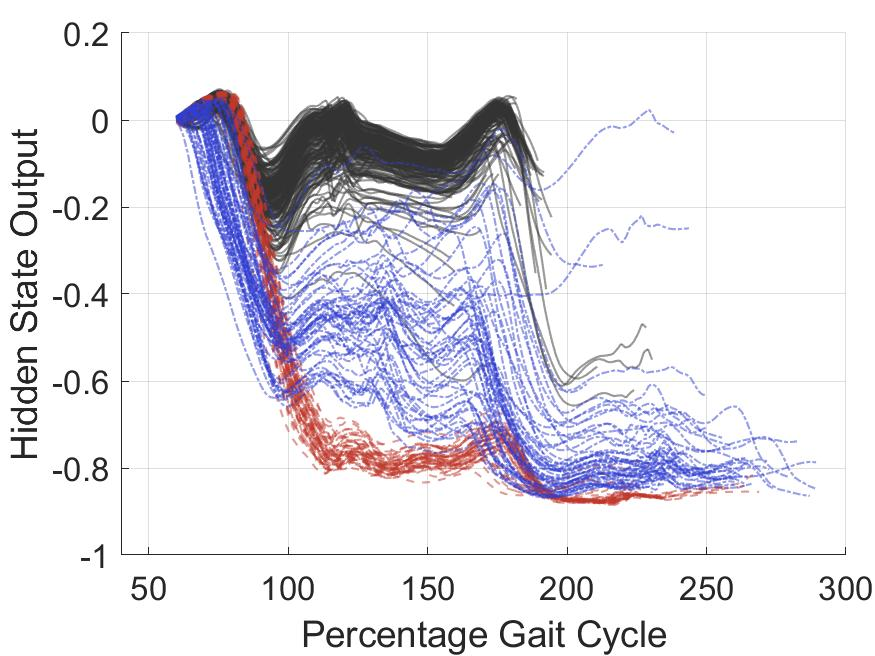
\includegraphics[width=\textwidth]{Figures/results/hidden_state/accel_x_w_v_sa-sd/60_Participant_04.jpg}
         \caption{60\%}
         \label{subfig:d}
     \end{subfigure}
     \hspace{0.5em}
     \begin{subfigure}[b]{0.32\textwidth}
         \centering
         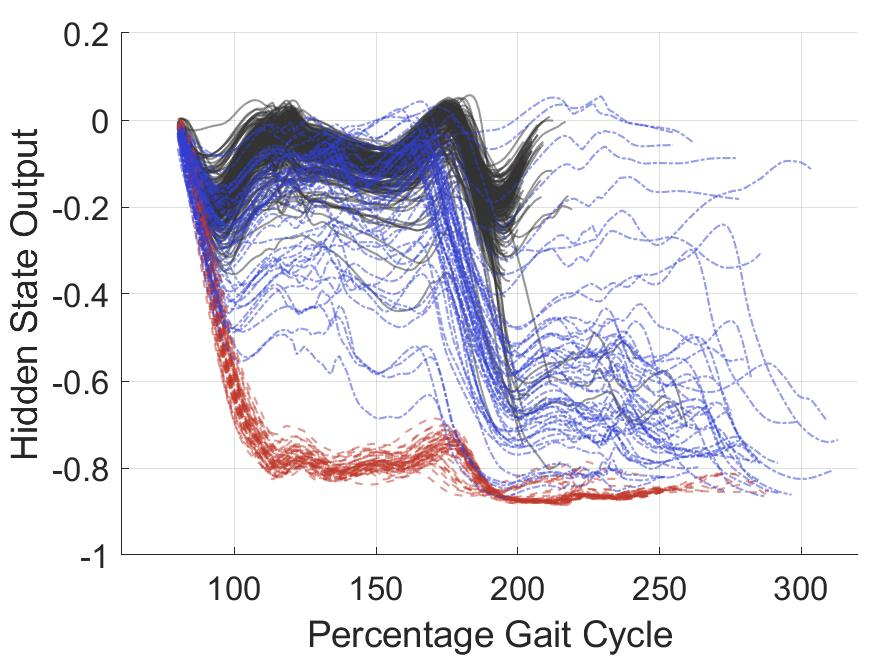
\includegraphics[width=\textwidth]{Figures/results/hidden_state/accel_x_w_v_sa-sd/80_Participant_04.jpg}
         \caption{80\%}
         \label{subfig:e}
     \end{subfigure}
    \caption{Hidden state of single unit LSTM model with x axis accelerometer as it's input. The model output classifies walking from stairs (ascent and stair descent). walking (blue), stair ascent (green) and stair descent (orange)}
    \label{fig:hidden-state-accel-x-w_v_sa-sd}
\end{figure}

For both acceleration and gyroscope the hidden state value changes most during swing and early stance. For the y gyroscope it can be seen that the classification of stair ascent from walking and stair descent occurs around 50\% gait cycle. From the gait trends this is about the point the gyroscope signals begin to converge. 

With the x accelerometer as in input there is less tightly grouped hidden state trends, correlates well with the higher standard deviation. Stair descent is less certain and the model struggles to separate it from walking. Stair ascent and walking are easily classified. Classification occurs around early swing.

No gain from having a window size greater than one step, classification only occurs in one phase of the cycle. It appear that to gain higher accuracy the model would need to learn more personalised information. For both input signals a similar behaviour was observed for all the output class sets.

%%%%%%%%%%%%%%%%%%%%%%%%%%%%%%%%%%%%%%%%%%%%%%%%%%%%%%%%%%%%%%%%%%%%%%%%%%%%%%%%%%%%%%%%%%%%%%%%%%%
 \subsection{Full Problem}%<TK>
The following section presents the results of investigations into how model performance changes with adjustments of hyper-parameters. The hyper-parameters selected for this were; network shape, input window size, unit width, depth, the number of inputs, varying sensors and axis, and number of participants.

For network size three different window sizes (32, 64 and 128 timesteps) and size different unit widths (4, 6, 8, 16, 32, 64) were tested. Each model shape was trained five times for the five different train/test data sets. Table \ref{tab:model_size_hyper_param} presents the model accuracy achieved for each models $\pm$ standard deviation. Table \ref{tab:model_size_hyper_param_train} and \ref{tab:model_size_hyper_param_test} show the validation and unseen participant test accuracy respectively for each configuration.

\begin{table}[!hbt]
    \centering
    \caption{Model accuracy for hyper-parameters for layer units and input window size for both seen and novel subjects}
    \label{tab:model_size_hyper_param}
    \begin{subtable}{.49\linewidth}
        \centering
        \caption{Accuracy for seen validation data}
        \label{tab:model_size_hyper_param_train}
        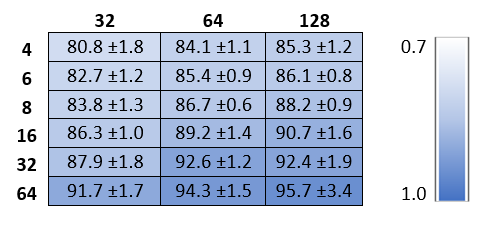
\includegraphics[width=\textwidth]{Figures/results/LSTM_Train_Accuracy.png}
    \end{subtable}
    \hfil
    \begin{subtable}{.49\linewidth}
        \centering
        \caption{Accuracy for unseen test data}
        \label{tab:model_size_hyper_param_test}
        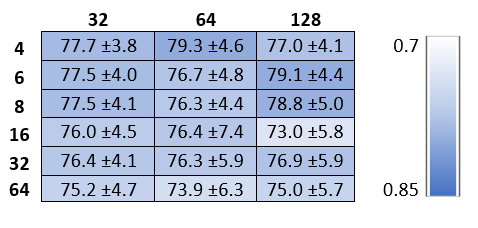
\includegraphics[width=\textwidth]{Figures/results/LSTM_Test_Accuracy.png}
    \end{subtable}
\end{table}

The validation accuracy increases with increasing model size. the improvement when moving from a 32 timestep widow to 64 is much greater than when increasing to 128. For test accuracy the results plateau around 80\%, after which the improvements in performance likely occur due to over fitting to the training data. This also corresponds with an increase in standard deviation.

Networks with 2-4 deep LSTM layers were tested but this showed no improvement in generalisation and only a small improvement in validation accuracy. The same was observed with multiple sensors there was no additional improvement in generalisation beyond a 6-axis IMU only an improvement in seen data accuracy.

%%%%%%%%%%%%%%%%%%%%%%%%%%%%%%%%%%%%%%%%%%
Figure \ref{fig:subject_num_generalisation} presents the changes in accuracy for varying number of participants used during training. The red line represents the smoothed novel test subject accuracy average for the ten models trained. The blue line represents the same for the training validation data. The solid area represent the standard deviation. Between 1 and 20 training subjects were used with a single excluded participant used for evaluating unseen data performance. Figure \ref{fig:subject_num_generalisation_64x12} and \ref{fig:subject_num_generalisation_128x6} show the results for a 64 timestep 12 unit and 128 time step 6 unit models respectively.

\begin{figure}[!htb]
    \centering
    \begin{subfigure}[b]{0.49\textwidth}
         \centering
        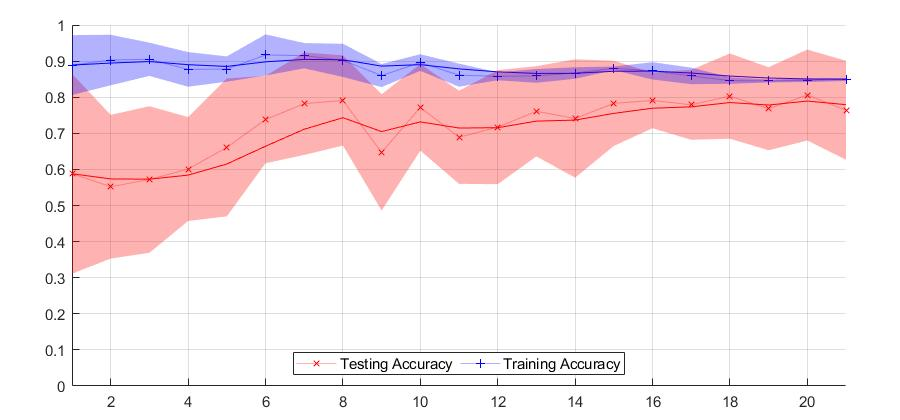
\includegraphics[width=\textwidth]{Figures/results/number_participants_64x12.jpg}
        \caption{64 Timesteps, 12 Units}
        \label{fig:subject_num_generalisation_64x12}
    \end{subfigure}
    \hfil
    \begin{subfigure}[b]{0.49\textwidth}
         \centering
        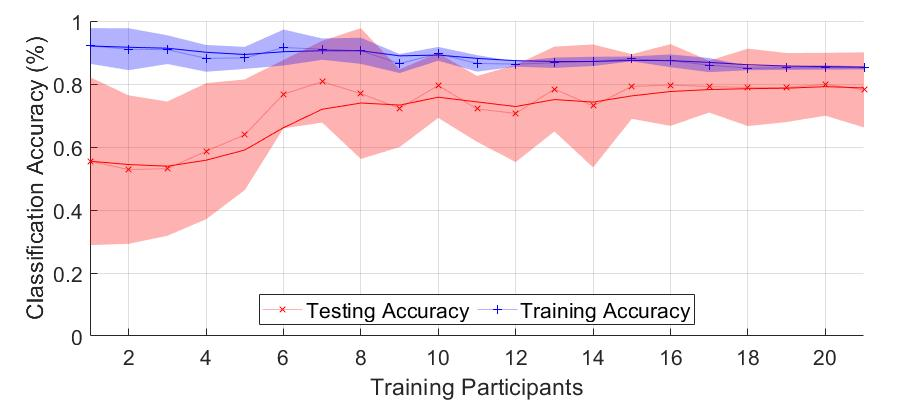
\includegraphics[width=\textwidth]{Figures/results/number_participants_128x6.jpg}
        \caption{128 Timesteps, 6 Units}
        \label{fig:subject_num_generalisation_128x6}
    \end{subfigure}
    \caption{Classification accuracy of seen/unseen subjects for training with different numbers of participants for two different models}
    \label{fig:subject_num_generalisation}
\end{figure}

Figure \ref{fig:subject_num_generalisation} shows that increasing the number of participants leads to better generalised performance, however the effects on increasing numbers of participants levels off around 15 participants. This would indicate that for novel subjects to achieve the high levels of classification performance that are possible with an LSTM increasing the number of subjects alone may not be enough.

%%%%%%%%%%%%%%%%%%%%%%%%%%%%%%%%%%%%%%%%%%
Table \ref{tab:128x6_full_model_confusion_matrix} shows the confusion matrices for a 128 timestep, 6 unit single layer LSTM network. Table \ref{tab:full_model_conf_matrix_training_128x6} is for the training validation data and Table \ref{tab:full_model_conf_matrix_test_128x6} the unseen test data. Table \ref{tab:128x32_full_model_confusion_matrix} shows the same for a model with 32 units. The 6 unit model had a overall classification accuracy of 87.4\% for validation and 84.7\% for test, the 32 unit model accuracy was 96.1\% and 76.0\%.

\begin{table}[!hbt]
    \centering
    \caption{128 timestep, 6 unit confusion matrices}
    \label{tab:128x6_full_model_confusion_matrix}
    \begin{subtable}{.45\textwidth}
        \centering
        \caption{Validation}
        \label{tab:full_model_conf_matrix_training_128x6}
        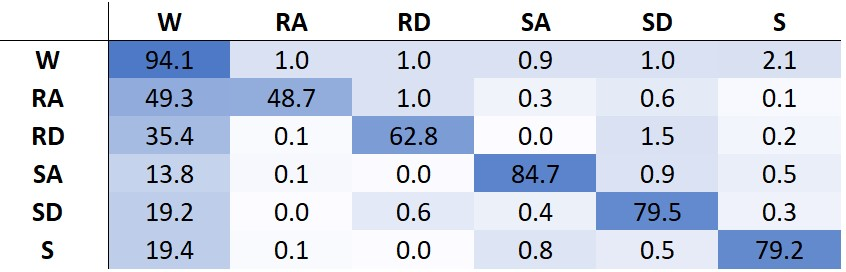
\includegraphics[width=\textwidth]{Figures/results/conf_matricies/Training_128x6_NT.jpg}
    \end{subtable}
    \hfil
    \begin{subtable}{.45\textwidth}
        \centering
        \caption{Test}
        \label{tab:full_model_conf_matrix_test_128x6}
        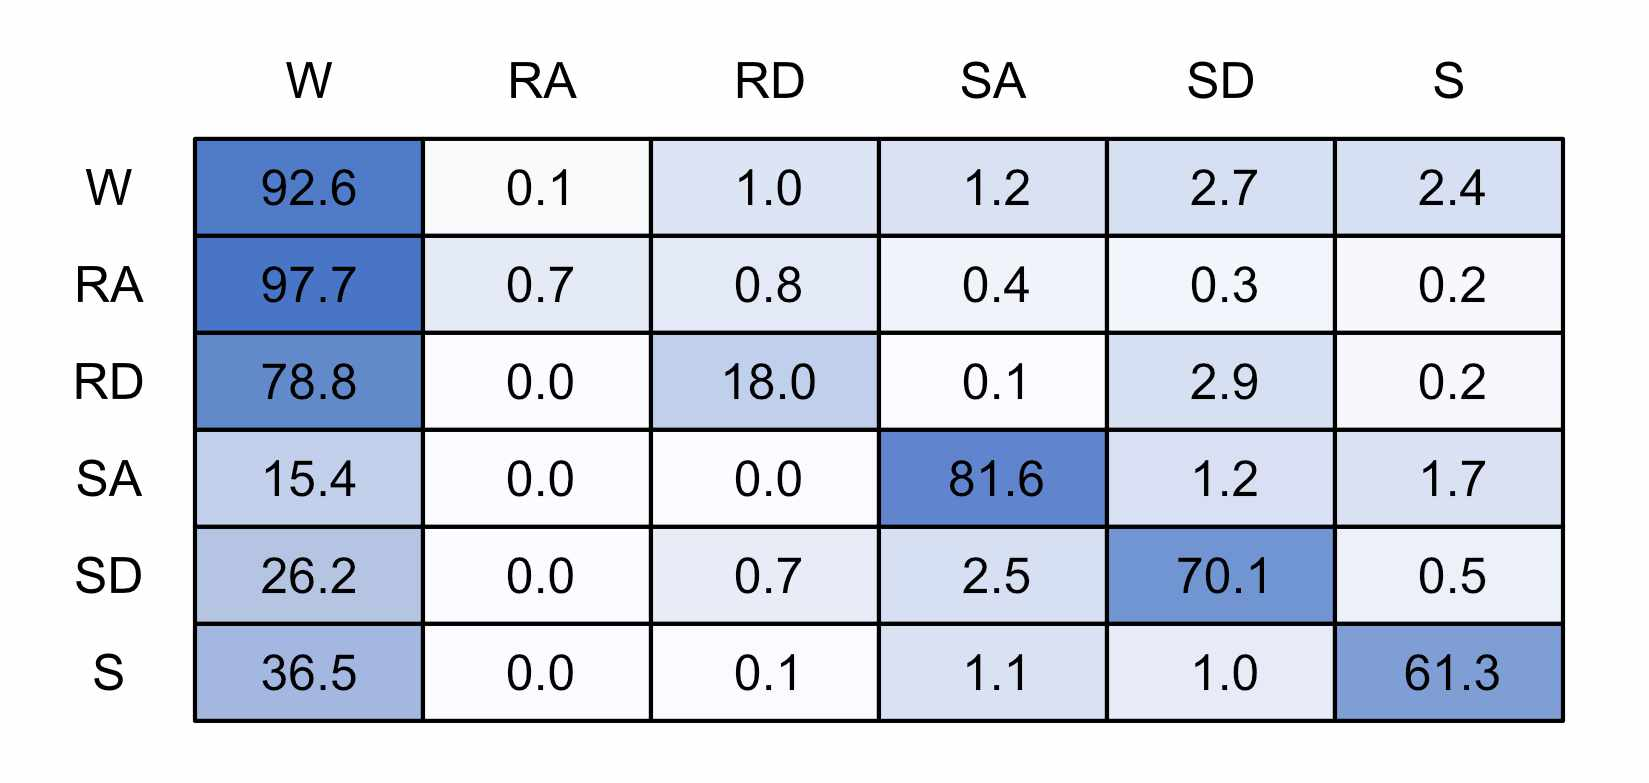
\includegraphics[width=\textwidth]{Figures/results/conf_matricies/Test_128x6_NT.jpg}
    \end{subtable}
\end{table}

\begin{table}[!hbt]
    \centering
    \caption{128 timestep, 32 unit confusion matrices}
    \label{tab:128x32_full_model_confusion_matrix}
    \begin{subtable}{.45\textwidth}
        \centering
        \caption{Validation}
        \label{tab:full_model_conf_matrix_training_128x32}
        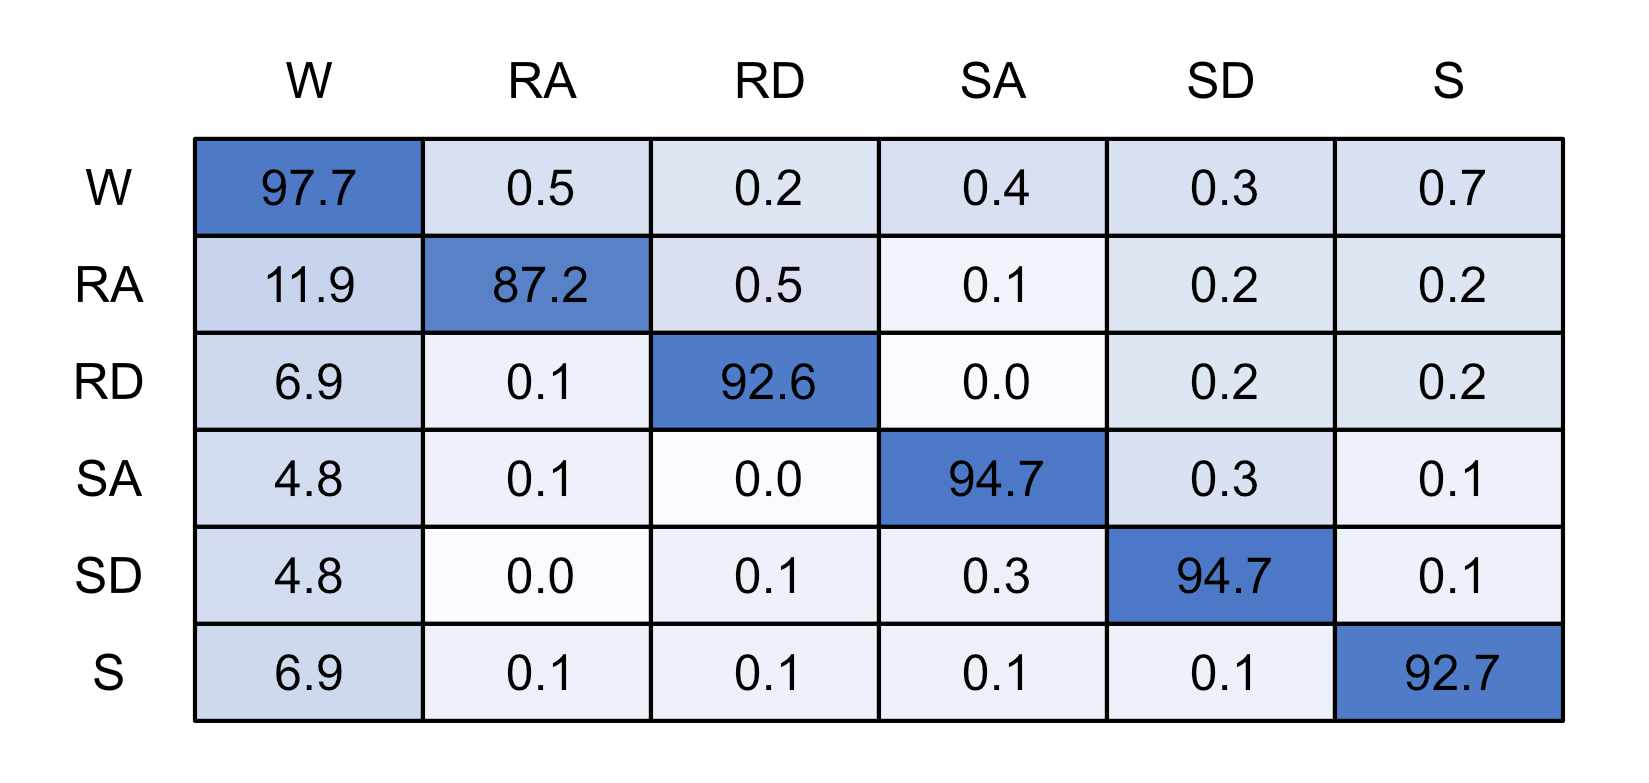
\includegraphics[width=\textwidth]{Figures/results/conf_matricies/Training_128x32_NT.jpg}
    \end{subtable}
    \hfil
    \begin{subtable}{.45\textwidth}
        \centering
        \caption{Test}
        \label{tab:full_model_conf_matrix_test_128x32}
        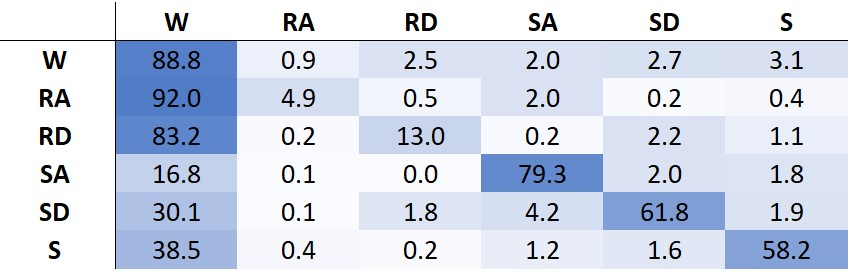
\includegraphics[width=\textwidth]{Figures/results/conf_matricies/Test_128x32_NT.jpg}
    \end{subtable}
\end{table}

It can be seen that nearly all miss-classifications are a confusion with walking. The test data showed a similar patterns for both models even though the 32 unit model is over-fitted to the training data. Some miss-classifications will be due to under labelled or discrepancies in point of labeling during recording.

Ramp descent and ascent the most confused. This is likely because of the similarities in gait cycle between the two activities and the difficulty is accurately labelling this activity due to subject biases on what constitutes a ramp. Stairs get slightly confused between each other but again mostly with walking. Stair Descent performs worse than stair ascent again this is likely due to it's closer gait shape to walking. It's not obvious why stop performs poorly.

%%%%%%%%%%%%%%%%%%%%%%%%%%%%%%%%%%%%%%%%%%

Figure \ref{fig:missclassification} shows a visual representation of the activities labelled during a recording above which is a plot of where the classification errors occur ed during that recording. As can be seen a large proportion of miss-classification occur around changes in activity. The transition between activities is highly varied.

\begin{figure}[!htb]
    \centering
    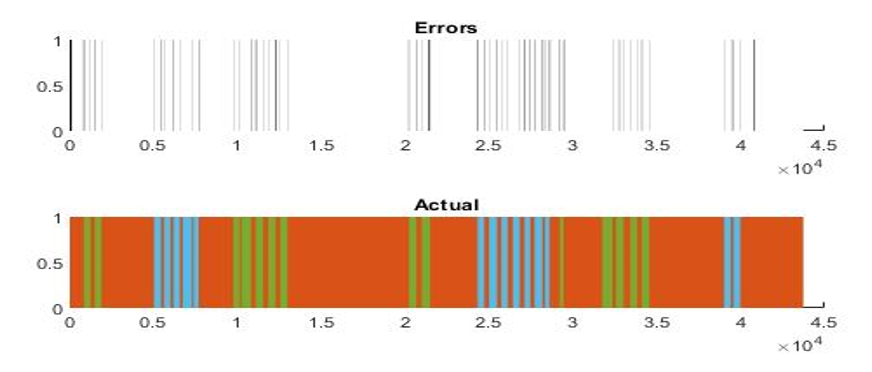
\includegraphics[width=0.8\textwidth]{Figures/results/Screenshot 2020-12-02 130339.png}
    \caption{Miss-classifications and labelled activity locations}
    \label{fig:missclassification}
\end{figure}

\section{Improving Novel User Performance}
From the above analysis it can be seen that the model performed more poorly when presented with new data in particular around changes in activity. To try and improve this an additional transition state was added to the model

% Methodology
The transition state was added to the classification output and the label data augmented with a transition region added for 0.5 seconds before and after changes in activity. A model was then trained again using the excluded participant cross validation to establish generalisation performance. Two model were trained with 128 time steps and 6 and 32 unit.

% Results
Tables \ref{tab:128x6_transition_confusion_matrix} and \ref{tab:128x32_transition_confusion_matrix} present the confusion matrices for the transition models trained with 6 and 32 units respectively. The 6 unit model achieved 82.8\% accuracy on validation data and 72.4\% for test, and the 32 unit model achieved 93.1\% and 69.3\%. If the transition state is excluded from the classification accuracy then when presented with test data the models achieve 75.2\% and 75.0\% accuracy for the 6 and 32 unit models respectively

\begin{table}[!hbt]
    \centering
    \caption{128x6 Transition Model}
    \label{tab:128x6_transition_confusion_matrix}
    \begin{subtable}{.45\textwidth}
        \centering
        \caption{Training}
        \label{tab:tran_model_conf_matrix_training_128x6}
        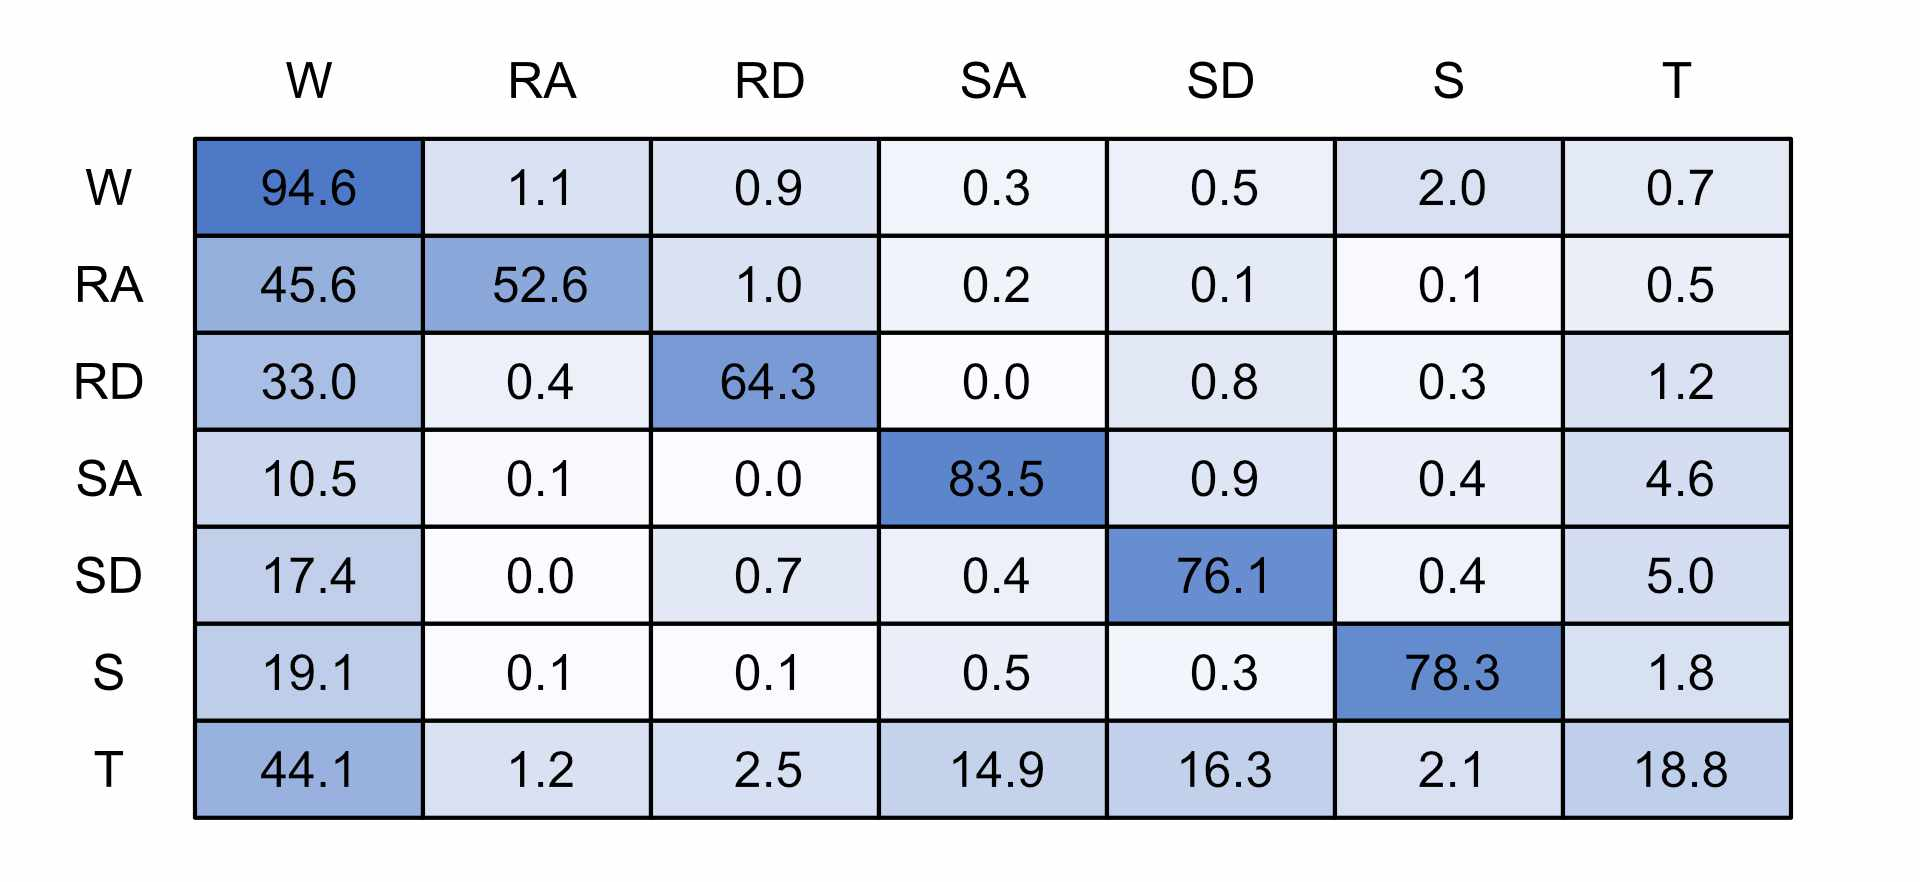
\includegraphics[width=\textwidth]{Figures/results/conf_matricies/Training_128x6_T.jpg}
    \end{subtable}
    \hfil
    \begin{subtable}{.45\textwidth}
        \centering
        \caption{Test}
        \label{tab:tran_model_conf_matrix_test_128x6}
        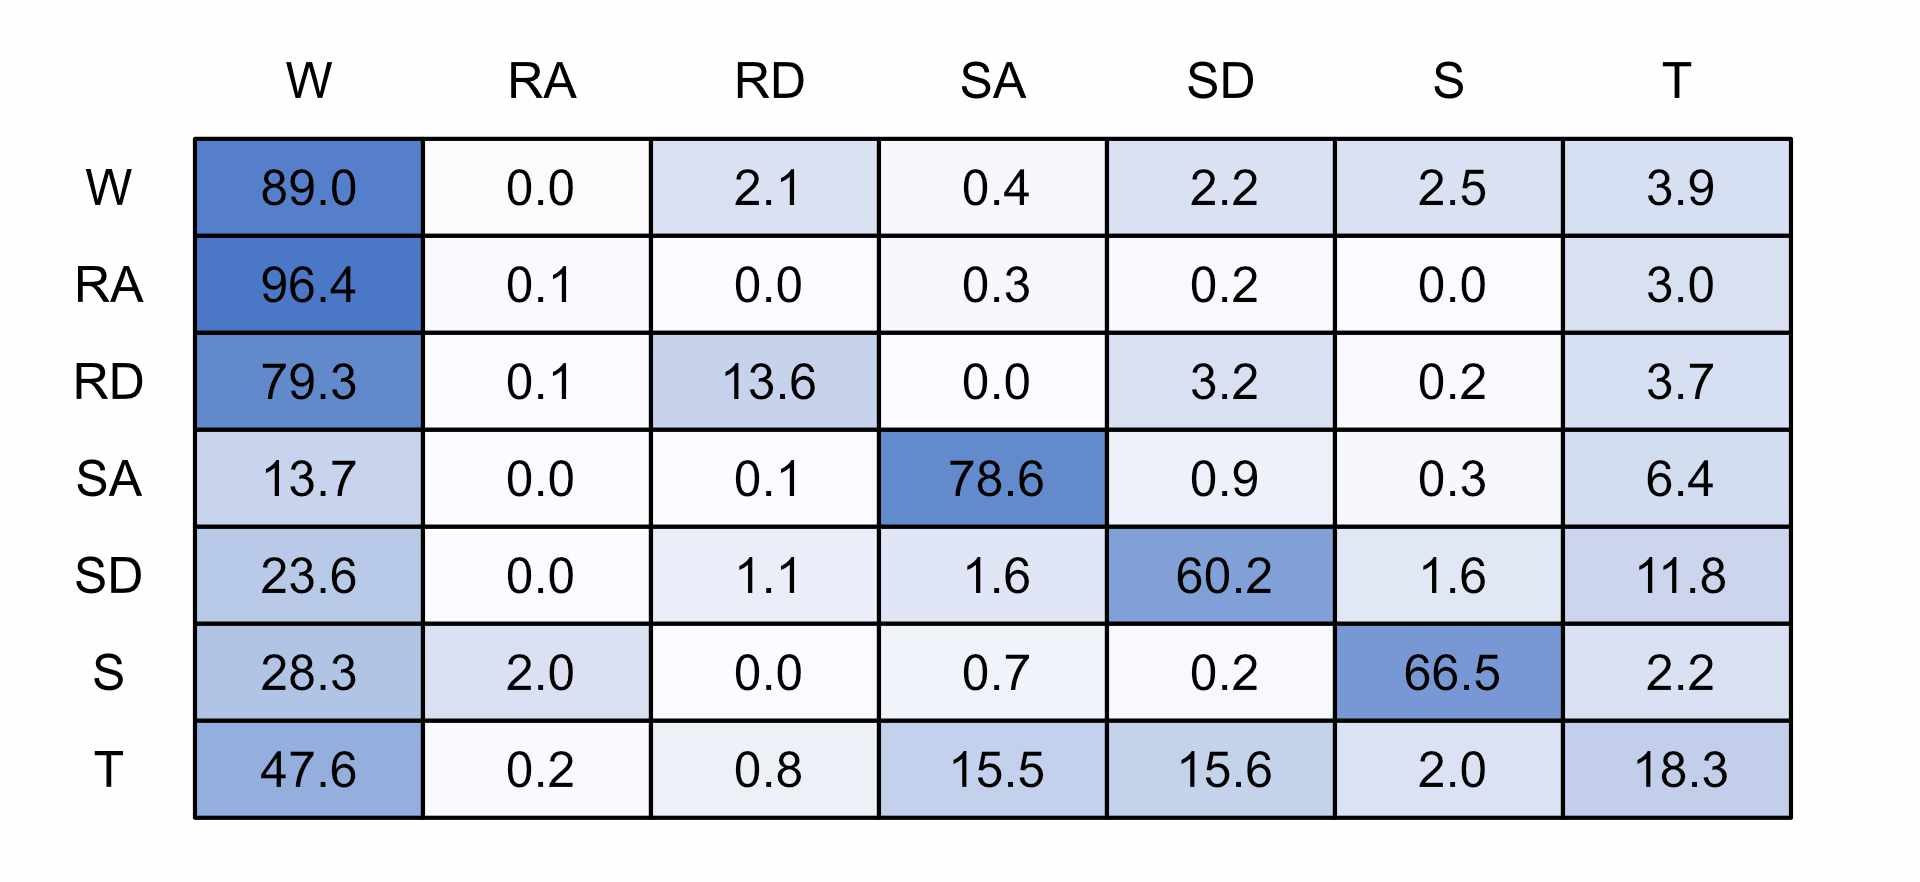
\includegraphics[width=\textwidth]{Figures/results/conf_matricies/Test_128x6_T.jpg}
    \end{subtable}
\end{table}

\begin{table}[!hbt]
    \centering
    \caption{128x6 Transition Model}
    \label{tab:128x32_transition_confusion_matrix}
    \begin{subtable}{.45\textwidth}
        \centering
        \caption{Training}
        \label{tab:tran_model_conf_matrix_training_128x32}
        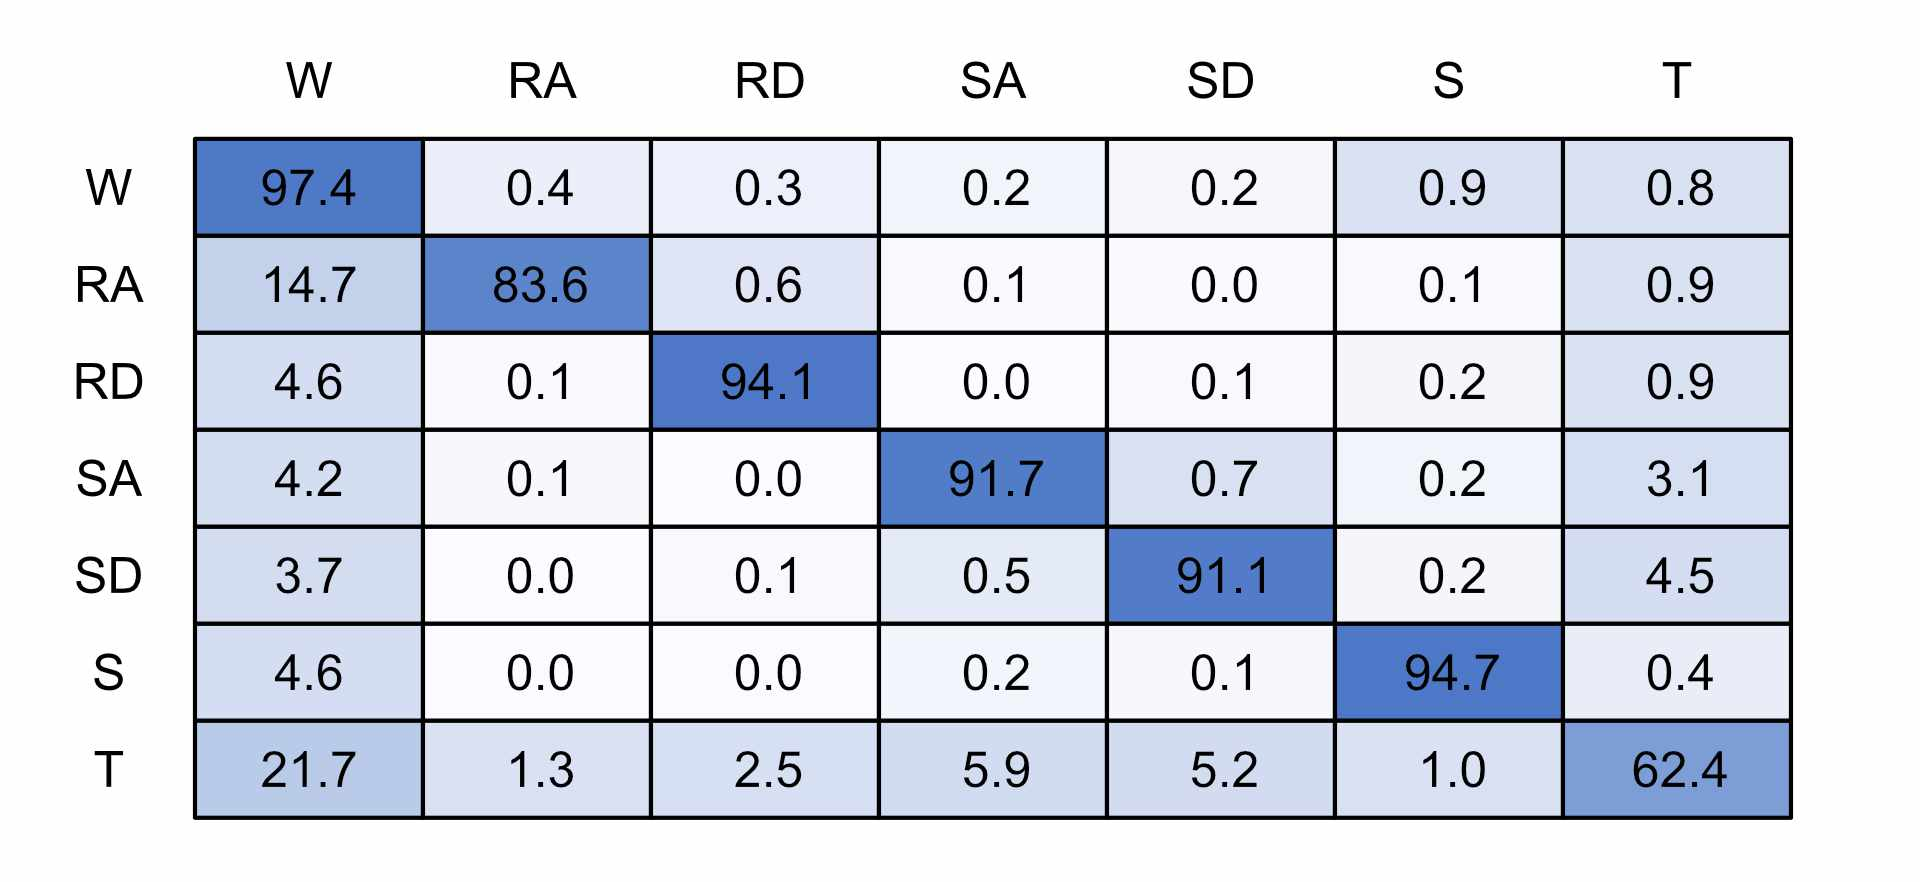
\includegraphics[width=\textwidth]{Figures/results/conf_matricies/Training_128x32_T.jpg}
    \end{subtable}
    \hfil
    \begin{subtable}{.45\textwidth}
        \centering
        \caption{Test}
        \label{tab:tran_model_conf_matrix_test_128x32}
        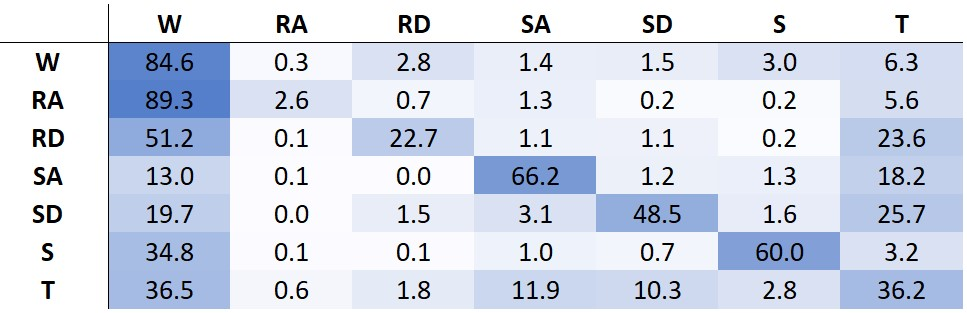
\includegraphics[width=\textwidth]{Figures/results/conf_matricies/Test_128x32_T.jpg}
    \end{subtable}
\end{table}

% Analysis
This method did not improve performance, equal or worse performance than without the transition state, even when excluding the transition state for classification accuracy. The transition region is highly uncertain and so the model will struggle to learn the expected behaviour.

%%%%%%%%%%%%%%%%%%%%%%%%%%%%%%%%%%%%%%%%%%
\section{Discussion}% TODO: Write up properly
%What did we learn from the simplified model and how was it useful in the full model?
The simplified model gave an insight into which areas of the gait cycle to model is likely to learn. The observations made from this appear to match up well with the larger model performance. Window size doesn't affect performance, as long as the window cover the stance phase the simplified model was able to identify the class. Therefore a window size of greater than one gait cycle offers no benefit as the last stance phase observed sets the final output. As was seen increasing subjects would not necessarily lead to a model that could generalise well to novel subject. As amputees have gaits that are much more varied between individuals this is significantly less likely to work.

The simplified model achieves high accuracy despite it's limited learning ability, albeit on a simplified problem. Therefore the higher accuracy achieved on the full model may in part be by learning the minute personal trends of the data for the participants. This may explain why the models struggle to generalise for new participants unless the model has been trained on a person with similar gait. 85\% appears to be an upper bound for LSTM using just IMU data when presenting novel users, instead of as Dehghani et al stated and over estimation of performance.

It was not really obvious why such deep models have been used in literature and they seem to offer negligible improvements in performance versus there size and result it models that very easily over fit.

The results of this work suggest that simply modifying adjusting the LSTM model hyper-parameters is not enough to produce a model that performs well with unseen users. Alternative approaches are therefore required to solve this problem. Additions to the output such smoothing to combine multiple classifications. Or more complex classifiers where more than just the maximum output value is used, instead classes are used establish how confident the model is. A system of personalisation could also be developed to adapt the model to an individual. It would be of interest to established whether a model trained from able-bodied users could be adapted to lower limb amputees.

%%%%%%%%%%%%%%%%%%%%%%%%%%%%%%%%%%%%%%%%%%
\section{Conclusions}% TODO: Write up properly
In this paper, we have presented a new data set for HAR research that...

We have investigated the behaviour of an LSTM using able-bodied subjects to provide suitable quantities of data. We have demonstrated that the learning is applicable to more complex models

Attempted to improve novel user performance by accounting for transitions between activities

Further work is still required in the areas
%Collect more data
%Investigate personalisation techniques
%Apply to amputee

%%%%%%%%%%%%%%%%%%%%%%%%%%%%%%%%%%%%%%%%%%
\vspace{6pt} 


%%%%%%%%%%%%%%%%%%%%%%%%%%%%%%%%%%%%%%%%%%
\authorcontributions{For research articles with several authors, a short paragraph specifying their individual contributions must be provided. The following statements should be used ``conceptualization, X.X. and Y.Y.; methodology, X.X.; software, X.X.; validation, X.X., Y.Y. and Z.Z.; formal analysis, X.X.; investigation, X.X.; resources, X.X.; data curation, X.X.; writing--original draft preparation, X.X.; writing--review and editing, X.X.; visualization, X.X.; supervision, X.X.; project administration, X.X.; funding acquisition, Y.Y.'', please turn to the  \href{http://img.mdpi.org/data/contributor-role-instruction.pdf}{CRediT taxonomy} for the term explanation. Authorship must be limited to those who have contributed substantially to the work reported.}

%%%%%%%%%%%%%%%%%%%%%%%%%%%%%%%%%%%%%%%%%%
\funding{Please add: ``This research received no external funding'' or ``This research was funded by NAME OF FUNDER grant number XXX.'' and  and ``The APC was funded by XXX''. Check carefully that the details given are accurate and use the standard spelling of funding agency names at \url{https://search.crossref.org/funding}, any errors may affect your future funding.}

%%%%%%%%%%%%%%%%%%%%%%%%%%%%%%%%%%%%%%%%%%
\acknowledgments{In this section you can acknowledge any support given which is not covered by the author contribution or funding sections. This may include administrative and technical support, or donations in kind (e.g., materials used for experiments).}

%%%%%%%%%%%%%%%%%%%%%%%%%%%%%%%%%%%%%%%%%%
\conflictsofinterest{The authors declare no conflict of interest. The funders had no role in the design of the study; in the collection, analyses, or interpretation of data; in the writing of the manuscript, or in the decision to publish the results.} 

%%%%%%%%%%%%%%%%%%%%%%%%%%%%%%%%%%%%%%%%%%
%% optional
\abbreviations{The following abbreviations are used in this manuscript:\\

\noindent 
\begin{tabular}{@{}ll}
HAR & Human Activity Recognition\\
ML & Machine Learning\\
LSTM & Long Short Term Memory\\
RNN & Recurrent Neural Network\\
\end{tabular}}

%%%%%%%%%%%%%%%%%%%%%%%%%%%%%%%%%%%%%%%%%%
%% optional
%%%%%%%%%%%%%%%%%%%%%%%%%%%%%%%%%%%%%%%%%%
% Citations and References in Supplementary files are permitted provided that they also appear in the reference list here. 

%=====================================
% References, variant B: external bibliography
%=====================================
\reftitle{References}
\externalbibliography{yes}
\bibliography{references}

%%%%%%%%%%%%%%%%%%%%%%%%%%%%%%%%%%%%%%%%%%
%% optional
%% for journal Sci
%\reviewreports{\\
%Reviewer 1 comments and authors’ response\\
%Reviewer 2 comments and authors’ response\\
%Reviewer 3 comments and authors’ response
%}

%%%%%%%%%%%%%%%%%%%%%%%%%%%%%%%%%%%%%%%%%%
\end{document}

